\chapter{Optimal coordinated yaw control of wind farms}\label{ch:opt_yaw}

\def\mystrut{\rule{0pt}{1.1\normalbaselineskip}}

The current chapter investigates optimal coordinated yaw control in wind farms. In the introduction, the concept of redirecting wakes using a steady and intentional yaw misalignment in upstream turbines was already introduced, and the prevalence of research on the characterization and exploitation of wake behavior behind turbines in steady yaw was shown. The application of dynamic optimal yaw control in the current chapter however allows to assess whether unsteady yaw behavior can yield improvements in power production due to benign interactions with the flow field. To the best knowledge of the author, this is the first time that this possibility is investigated. Furthermore, the potential of combining dynamic yaw control with dynamic induction control is examined. Control studies are performed for a wind farm of 16 turbines layed out in a $4 \times 4$ aligned pattern, both for a uniform inflow and a turbulent boundary layer inflow. 

The outline of the chapter is as follows. Section~\ref{sec:opt_yaw_setup} describes the simulation cases, and details numeral setup parameters. Thereafter, Section~\ref{sec:opt_yaw_results} presents optimization results for both uniform and turbulent inflow, and identifies distinct yaw control regimes resulting in increased power extraction. Finally, Section~\ref{sec:opt_yaw_concl} summarizes the main findings of the current chapter. 

Parts of the content of this chapter have been submitted for publication in the paper Munters \& Meyers, ``Dynamic strategies for yaw and induction control of wind farms based on large-eddy simulation and optimization''.


\section{Numerical setup and case description}\label{sec:opt_yaw_setup}
This section discusses the simulation cases and setup details that will be used to assess the potential of dynamic yaw control. A wind farm of 16 wind turbines with a rotor diameter $D = 100$ m is considered. The turbines are arranged in a $4 \times 4$ aligned pattern, with $6D$ spacing in both axial and transversal directions. Firstly, the specific optimization problem considered in the current chapter is detailed. Afterwards, numerical setup parameters for the simulation and optimization are discussed. Finally, the different control cases are introduced. 

\subsubsection{Optimization problem}
The optimal control studies in the current chapter involve both dynamic induction and dynamic yaw, hence the optimization problem at hand is the full problem introduced in Chapter~\ref{ch:opt_formulation}, i.e. 
\begin{mini!}[1]
	{\scriptsize \bs{\varphi}, \bs{q}}{\J(\bs{\varphi}, \bs{q}) = - \Tint \sum_{i=1}^{N_t} \frac{1}{2} a \ctihat~V_i^3 A_i \dt}{\label{eq:yawcostfunction_inside_problem}}{}
	%	\addConstraint{\small \frac{\partial \utilde}{\partial t} + \big(\utilde \cdot \nabla \big)\utilde }{\small = - \nabla (\ptilde + \ptilde_\infty) / \rho - \nabla \cdot \boldsymbol{\tau}_{sgs} + \sum_{i=1}^{N_t} \bs{f}_i\ + \bs{f}_{\text{fr}} }{\small \text{in } \Omega \times (0,T] \label{eq:NSmomentum_constraint}}
	\addConstraint{\small \frac{\partial \utilde}{\partial t} + \big(\utilde \cdot \nabla \big)\utilde }{\small = - \nabla \ptilde / \rho - \nabla \cdot \boldsymbol{\tau}_{sgs} + \sum_{i=1}^{N_t} \bs{f}_i\ + \bs{f}_{\text{fr}}\ \ }{\small \text{in } \Omega \times (0,T] \label{eq:yawNSmomentum_constraint}}	
	\addConstraint{\small \nabla \cdot \utilde}{\small =0, \label{eq:yawNScontinuity_constraint}}{\small \text{in } \Omega \times (0,T]}
	\addConstraint{\small \tau \ddt{\ctihat}}{\small =\cti - \ctihat \label{eq:yawctihat_constraint}}{\small i=1...N_t~\text{in } (0,T]}
	\addConstraint{\small \ddt{\theta_i}}{\small = \omega_i \label{eq:yawomega_constraint}}{\small i=1...N_t~\text{in } (0,T]}
	\addConstraint{\small C_{T,\text{min}}' \leq}{\small  \cti \leq C_{T,\text{max}}' \label{eq:yawboxct_constraint}}{\small i=1...N_t~\text{in } (0,T]}
	\addConstraint{\small -\omega_{\text{max}} \leq}{\small  \omega_i \leq \omega_{\text{max}} \label{eq:yawboxomega_constraint}}{\small i=1...N_t~\text{in } (0,T],}
\end{mini!}
with system states $\bs{q}(\bs{x},t) = [\ufilt(\bs{x},t),\ \ptilde(\bs{x},t),\ \widehat{\bs{C}}_T'(t),\ \bs{\theta}(t)]$ and controls $\bs{\varphi}(t)~=~[\bs{C}_T'(t), \bs{\omega}(t)]$. The numerical values for $C_{T, \rm min}', \ctmax$, and $\omega_{\rm max}$ in the box constraints are given below in Table~\ref{tab:case_definition}.

\subsubsection{Simulation setup}
The simulation domain has a total dimension of $4.8 \times 2.4 \times 1 $ km$^3$, and is discretized on a grid of $256 \times 128 \times 128$ gridpoints. The final $10\%$ of the streamwise extent of the domain is used as a fringe region to impose inflow conditions. All cases apply periodic boundary conditions on transversal domain boundaries. 

Two different sets of simulations are considered. The first set is subjected to a steady and uniform inflow with $U_\infty = 8$ m s$^{-1}$. In this case, the top and bottom boundaries are treated with a symmetry condition, and the turbines are placed at the vertical mid-plane $z_h/H = 0.5$ to minimize any influence of vertical domain boundaries. The second set applies unsteady turbulent inflow conditions, which are generated in a pressure-driven precursor simulation of an unperturbed turbulent boundary layer driven by a pressure gradient of $\partial_x p_\infty/\rho = 2.5 \times 10^{-4}$ m s$^{-2}$ with shifted periodic boundary conditions, similar to the induction cases in Chapter~\ref{ch:opt_induction}. In this second case, the top boundary is treated with a stress-free condition, and a high-Reynolds number wall model is used at the bottom. The turbines are placed at a height of $z_h/H = 0.1$ from the wall. The wall model adds a wall stress consistent with a rough-wall logarithmic boundary layer profile with roughness length $z_0/H = 10^{-4}$, resulting in a inflow turbulence intensity of about 8\% at hub height. 

Within the context of the receding-horizon methodology introduced in Section~\ref{sec:problem_receding}, the optimization is performed over 6 time windows. Each window applies an optimization horizon $T=300$ s and a flow advancement time of $T_A = T/2= 150$ s, resulting in a total control time of 900 s. All time-averaged results shown below are based on statistics gathered after 300 s to compensate for the wake propagation time lag at startup. To limit computational efforts, we perform a fixed amount of 80 L--BFGS--B iterations in each window, corresponding to approximately 160 PDE simulations (forward or adjoint). Although formal convergence is not achieved for any of the cases after this amount of iterations, it will be shown later that the relative ordering of the cases based on power extraction is clear. Computational costs amount to approximately 35~000 corehours per optimization case for all 6 time windows combined on 112 Intel Broadwell architecture cores connected by an EDR Infiniband network. The initial guess for the optimal controls within each window is a steady thrust coefficient setpoint $C_T'=2$  and yaw rate $\omega = 0^\circ$ s$^{-1}$ for all turbines. Simulation and optimization parameters are summarized below in Table~\ref{tab:case_definition}.

Simulations are initialized as follows: for the turbulent inflow case, a fully-developed high-Reynolds number turbulent boundary layer is generated in the precursor inflow simulation by simulating a perturbed logarithmic flow until a statistically--stationary state is achieved. For both the turbulent and the uniform inflow cases the main wind-farm simulation is then advanced in time with the proper inflow conditions for approximately 5 wind-farm flow-through times, after which the effects of wind-farm start-up transients have subsided. These statistically stationary wind-farm flows then serve as initial conditions for the control cases defined below. Planviews at hub height of these initial conditions are shown in Figure~\ref{fig:initial_conditions_flow_yaw}. It can be seen from the Figure~\ref{fig:initial_conditions_flow_yaw}a that, given laminar inflow conditions, turbine wakes are very deep and remain stable up until row 3, after which meandering and vortex shedding starts to occur. These flow conditions can be regarded as somewhat artificial since, in the atmospheric boundary layer, background turbulence typically causes instant wake transition behind the turbine rotor. Nevertheless, this setup allows us to investigate control dynamics more easily, as we can rule out any reaction of the optimization to the background variability. Furthermore, suppressed wake meandering and reduced turbulence levels have been known to occur in wind farms submerged in stably stratified atmospheric boundary layers \citep{larsen2009dependence, machefaux2016experimental}, hence rendering the current case relevant for such situations. Figure~\ref{fig:initial_conditions_flow_yaw}b shows that, for the turbulent inflow case, the background turbulence causes wake instabilities instantly, leading to enhanced wake recovery and much more complex unsteady wake interactions between turbines.

\begin{figure}
	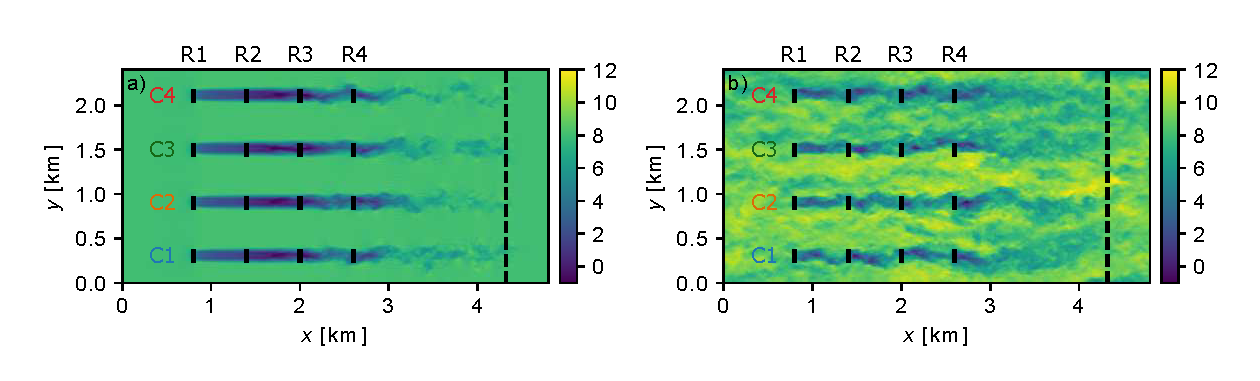
\includegraphics[width=\textwidth]{chapters/optimal_yaw_control/domain_rast_RC.eps}
	\caption[Planview at hub height $z_h$ of initial conditions for optimal control cases.]{Planview at hub height $z_h$ of initial conditions for optimal control cases. \emph{a)} Uniform and steady inflow. \emph{b)} Turbulent inflow. Colors represent instantaneous streamwise velocity $\widetilde{u}_x$ in m s$^{-1}$. The black lines represent wind turbine locations. The black dashed line indicates the start of the fringe region. R1 -- R4 and C1 -- C4 indicate the numbering convention used for turbine rows and columns respectively. \label{fig:initial_conditions_flow_yaw}}
\end{figure}

\subsubsection{Control cases}

For each set of simulations, a steady reference case (R) with $C_T' = 2$ and $\omega = 0^\circ s^{-1}$ is considered. Further, a first yaw control case (Y) is defined, with a steady $C_T'=2$, but turbines are allowed to yaw dynamically at a maximum rate of $\omega^{\text{max}} = 0.3^\circ s^{-1}$, corresponding to the maximum yaw rate of the conceptual NREL 5MW and the DOWEC 6MW turbines \citep{jonkman2009definition, kooijman2003dowec}. In addition, a second yaw control case (Y5) is constructed, for which a higher maximum yaw rate of $\omega^{\text{max}} = 5^\circ s^{-1}$ is selected. Although this significantly exceeds the capabilities of the abovementioned turbine design concepts, this case will allows to assess whether significant gains in power could be achieved by rapidly yawing turbine designs, such as low-inertia two-bladed teeter hinge wind turbines \citep{kim2014yaw}. 

Also, two induction control cases are considered, in which turbines can adapt their thrust coefficient $C_T'$ with a characteristic time scale $\tau = 5$ s: an underinductive case (I2, with $\ctmax = 2$), and an overinductive case (I3, with $\ctmax = 3$). Finally, for both the latter cases, also the option of combining dynamic induction control with the yaw control of case Y is considered, defining the yaw--induction cases I2Y and I3Y respectively. The cases investigated in this study are summarized in Table~\ref{tab:case_definition}. 

\begin{table}
	\caption{Setup parameters for optimal dynamic induction and yaw control cases \label{tab:case_definition}}
	\begin{tabular}{llccc}
		\hline 
		\multicolumn{5}{l}{\textbf{Simulation parameters}}\\
		Domain size  			& \multicolumn{4}{l}{$L_x \times L_y \times H = 4.8 \times 2.4 \times 1$ km$^3$}  \\ 
		Turbine dimensions  		& \multicolumn{4}{l}{$D = 0.1H = 100$ m}\\ 
		Turbine spacing  		& \multicolumn{4}{l}{$S_x = 6D, \quad S_y = 6D$}\\
		Windfarm layout 		& \multicolumn{4}{l}{$N_t = 16 $ turbines = 4 rows $\times$ 4 columns} \\ 
		Grid size 			& \multicolumn{4}{l}{$N_x \times N_y \times N_z = 256 \times 128 \times 128$}\\
		Cell size 			& \multicolumn{4}{l}{$\Delta_x \times \Delta_y \times \Delta_z = 18.75 \times 18.75 \times 7.8$ m$^3$}\\
		Time step 			& \multicolumn{4}{l}{$\Delta t = 0.75$ s}\\		
		& & & & \\	
		\multicolumn{5}{l}{\textit{Uniform inflow}}\\
		Hub height & \multicolumn{4}{l}{$z_h/H$ = 0.5}\\
		Inflow velocity & \multicolumn{4}{l}{$U_\infty$ = 8 m s$^{-1}$}\\
		& & & & \\			
		\multicolumn{5}{l}{\textit{Turbulent inflow}}\\
		Hub height & \multicolumn{4}{l}{$z_h/H$ = 0.1}\\		
		Precursor pressure gradient  	& \multicolumn{4}{l}{$ \partial_x p_\infty = 2.5 \times 10^{-4}$ m s$^{-2}$}  \\ 
		Surface roughness  &  \multicolumn{4}{l}{$z_0 = 10^{-4}H = 0.1$ m}\\ 		
		& & & & \\	
		\multicolumn{5}{l}{\textbf{Optimization parameters}}\\
		Optimization method		& \multicolumn{4}{l}{L--BFGS--B} \\
		Hessian correction pairs	& \multicolumn{4}{l}{$m = 5$} \\
		BFGS iterations 		& \multicolumn{4}{l}{$N_{it} = 80$ ($\approx 160$ PDE)} \\
		Optimization time window	& \multicolumn{4}{l}{$T = 300$ s}\\
		Flow advancement time window 	& \multicolumn{4}{l}{$T_A = 150$ s}\\
		Total operation time         	& \multicolumn{4}{l}{$T_{tot} = 900$ s (6 windows)}\\
		& & & & \\	
		\textbf{Cases} & \  & $C_{T,\text{min}}'$ & $C_{T,\text{max}}'$ & $\omega_{\text{max}}$ [$^\circ s^{-1}$] \\ 
		Reference & (R)    &  2 & 2 & 0   \\ 
		Yaw control & (Y)   &  2 & 2 & \textbf{0.3} \\ 
		Fast yaw control & (Y5)   &  2 & 2 &\textbf{5}   \\ 
		Underinduction control & (I2)    &  \textbf{0} & 2 & 0\\
		Overinduction control & (I3)    &  \textbf{0} & \textbf{3} & 0\\ 
		Underinduction + yaw control & (I2Y)   &  \textbf{0} & 2 & \textbf{0.3} \\ 
		Overinduction + yaw control & (I3Y)   &  \textbf{0} & \textbf{3} & \textbf{0.3} \\ 
		\hline 
	\end{tabular} 
\end{table}









\section{Results \& discussion}\label{sec:opt_yaw_results}
The current section presents and discusses the results of the optimal control cases. Firstly, the convergence behavior is illustrated for a typical optimization window, justifying the optimization parameters discussed in previous section. Thereafter, Section~\ref{sec:opt_yaw_uniform} and~\ref{sec:opt_yaw_turb} present the results of the uniform and turbulent inflow cases respectively. Concluding, Section~\ref{sec:opt_yaw_disc} compares both simulation sets and identifies the most promising control approaches.

Figure~\ref{fig:convergence} illustrates the typical convergence behavior within an optimization window for the uniform inflow case. Figure~\ref{fig:convergence}a shows that, although formal convergence is not achieved for any of the cases, after 80 iterations, the relative ordering of the cases is clear and further improvements in the cost function for an increased amount of iterations are marginal. From Figure~\ref{fig:convergence}b it can be seen that the amount of PDE evaluations (forward or adjoint) is approximately twice the amount of BFGS iterations, indicating that the optimizer mostly takes Newton steps without a further line search. Furthermore, similar to the behavior of the exclusively inductive cases from Chapter~\ref{ch:opt_induction}, the strong increase in PDE evaluations for I3 and I2Y can be explained by the fact that the limits of continuous adjoint gradient accuracy complicate satisfaction of the Wolfe conditions upon approaching a (local) optimum. Similar characteristics were observed for the turbulent case (not further shown here).

\begin{figure}
	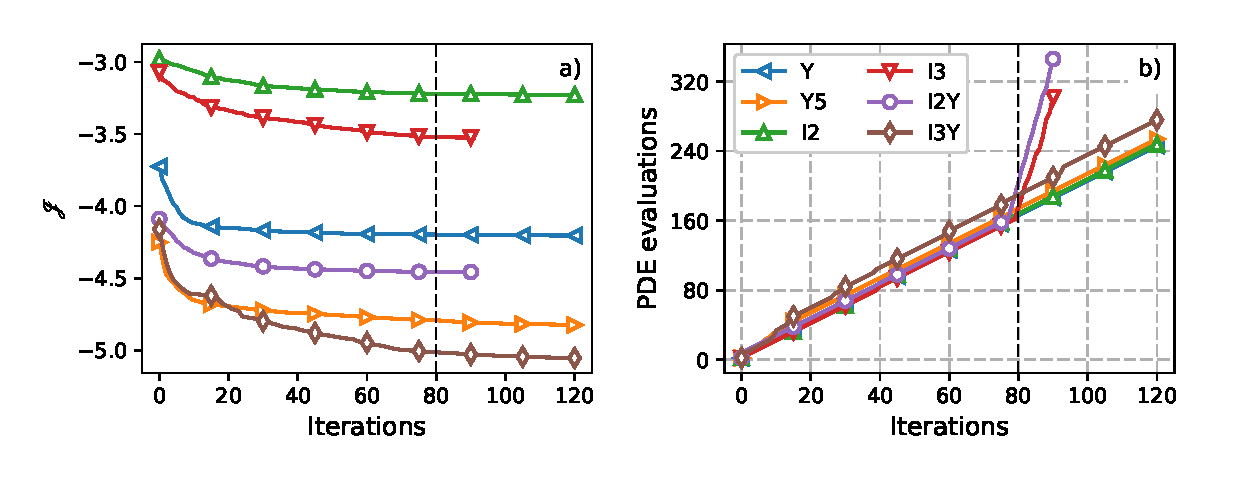
\includegraphics[width=\textwidth]{chapters/optimal_yaw_control/convergence_cost_pde.eps}
	\caption[Typical convergence behavior within an optimization window for uniform inflow.]{Typical convergence behavior within an optimization window for uniform inflow. \emph{a) }: Cost functional $\mathscr{J}$. \emph{b) }: PDE evaluations (forward or adjoint). Markers represent every fifteenth iteration step.\label{fig:convergence}}
\end{figure}

\subsection{Uniform inflow}\label{sec:opt_yaw_uniform}

	Figure~\ref{fig:flowfield_uniform} depicts instantaneous planviews of velocity and vorticity at hub height at t = 450 s for the reference case R, yawing case Y, overinductive case I3, and combined case I3Y. A first qualitative comparison between the flow fields indicates that, for the given setup, case Y achieves more intense wake mixing, destabilization, and lateral spreading through reorientation of turbine thrust forces than the overinductive case I3, which attempts to increase mixing by shedding vortex rings (similar to the process observed in Chapter~\ref{ch:opt_analysis}). Furthermore, the combined case I3Y shows a superposition of the aforementioned behavior, i.e. redirected wakes with periodically shed vortices. 
	
	\begin{figure}
		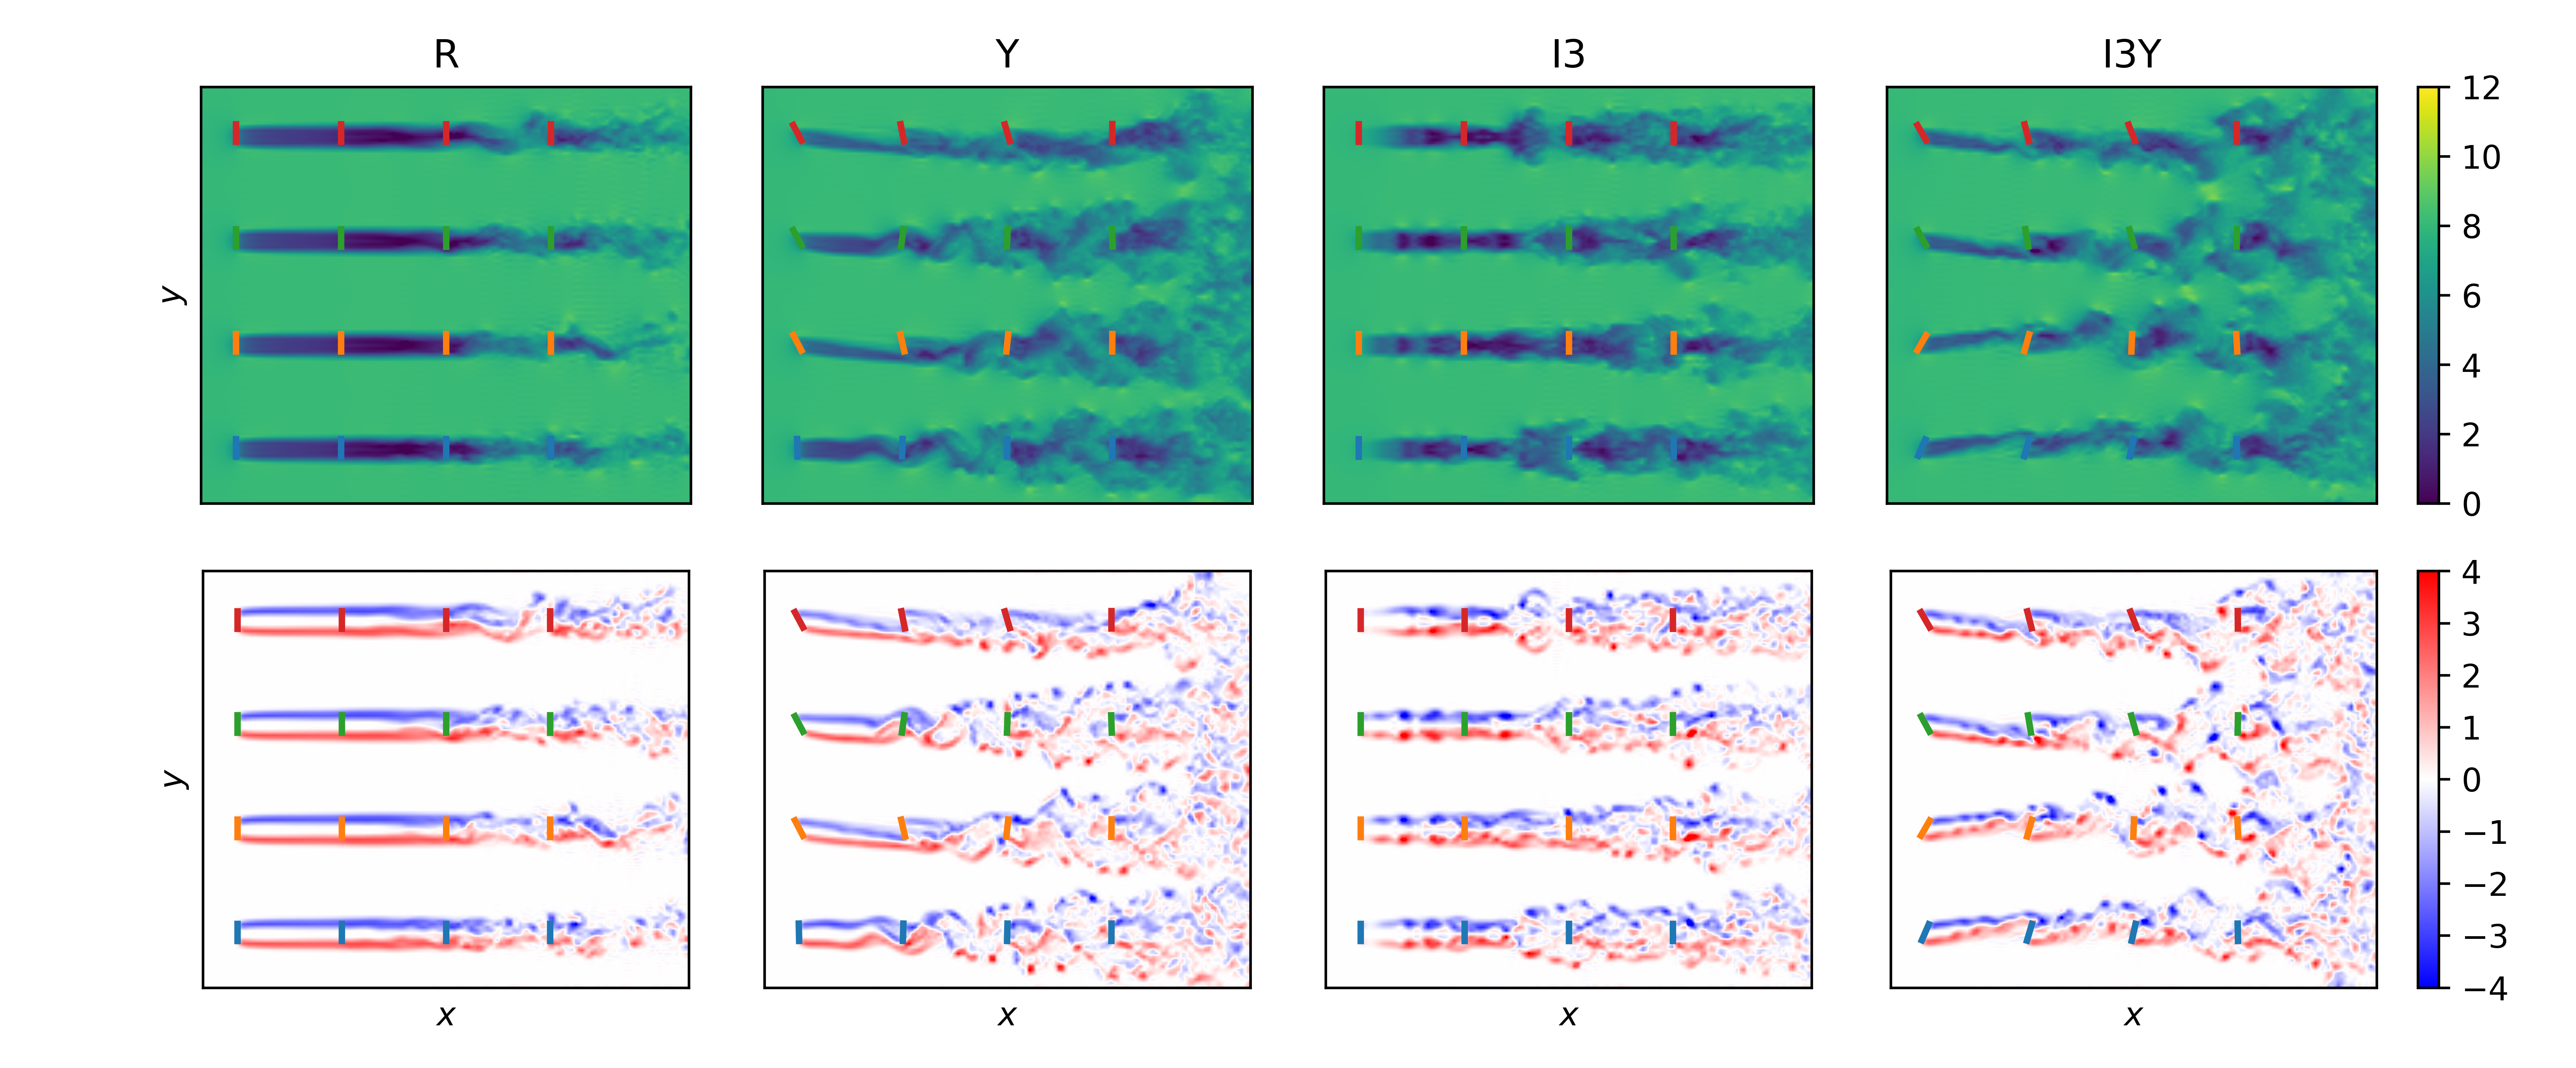
\includegraphics[width=\textwidth]{chapters/optimal_yaw_control/flow_field_lam.eps}
		\caption[Instantaneous planviews at hub height for uniform inflow cases R, Y, I3, and I3Y at $t= 450$ s.]{Instantaneous planviews at hub height for uniform inflow cases R, Y, I3, and I3Y at $t= 450$ s. \emph{Top: } Streamwise velocity. \emph{Bottom: } Wall-normal vorticity. Coloring is in units of m s$^{-1}$, s$^{-1}$. \label{fig:flowfield_uniform}}
	\end{figure}
	
	First, time-averaged power extraction and wind-farm efficiency are compared between cases. Second, yaw characteristics of the yaw-enabled control cases Y, Y5, I2Y, and I3Y are discussed. Time evolution of yaw angles are shown, and two distinct yawing regimes are identified. Finally, the induction characteristics of induction-enabled cases I2, I3, I2Y, and I3Y are shortly presented.
	
	\subsubsection{A. Power extraction and wind-farm efficiency}
	
	Figure~\ref{fig:power_uniform} illustrates time-averaged wind-farm power. Figure~\ref{fig:power_uniform}a shows row-averaged power extraction of the optimal control and reference cases, normalized by first-row reference power $\overline{P}_{R1}^R$. It is shown that all cases curtail first-row power by about $10-20\%$ to the benefit of downstream rows. Furthermore, yawing cases Y, Y5, I2Y and I3Y achieve an almost flat power curve among rows, and significantly outperform the inductive cases I2 and I3, for which modest gains are obtained only in the second and third row. Note the last row of I3Y, achieving  power extraction close to freestream conditions.
	
	Figure~\ref{fig:power_uniform}b depicts the wind farm efficiency, defined with respect to a situation in which all turbines extract the same power as a first-row reference case turbine, i.e. $\eta_{\text{farm}} = \overline{P}_{\text{farm}}/(N_t \overline{P}_{R1}^{R})$. As expected, the efficiency of the uncontrolled reference farm R is very low at around $40\%$. The inductive cases I2 and I3 manage to increase the efficiency to approximately 50\%, whereas the standard yawing case Y attains an overall efficiency of about 77$\%$. Further, it can be seen that, under uniform inflow conditions, adding the possibility of fast yawing (case Y5) or underinduction (case I2Y) yields only a very minor increase in wind-farm efficiency. In contrast, the combined overinductive yaw control from case I3Y results in a significantly higher efficiency of about 84\%, indicating the potential for combining these control strategies under uniform inflow. The figure also includes results for two additional control cases Ystat and Ymndr, based on simplified controls derived from yaw characteristics of the optimal control cases. These simplified cases are further detailed and discussed below.
	
	   
	
	
	\begin{figure}
		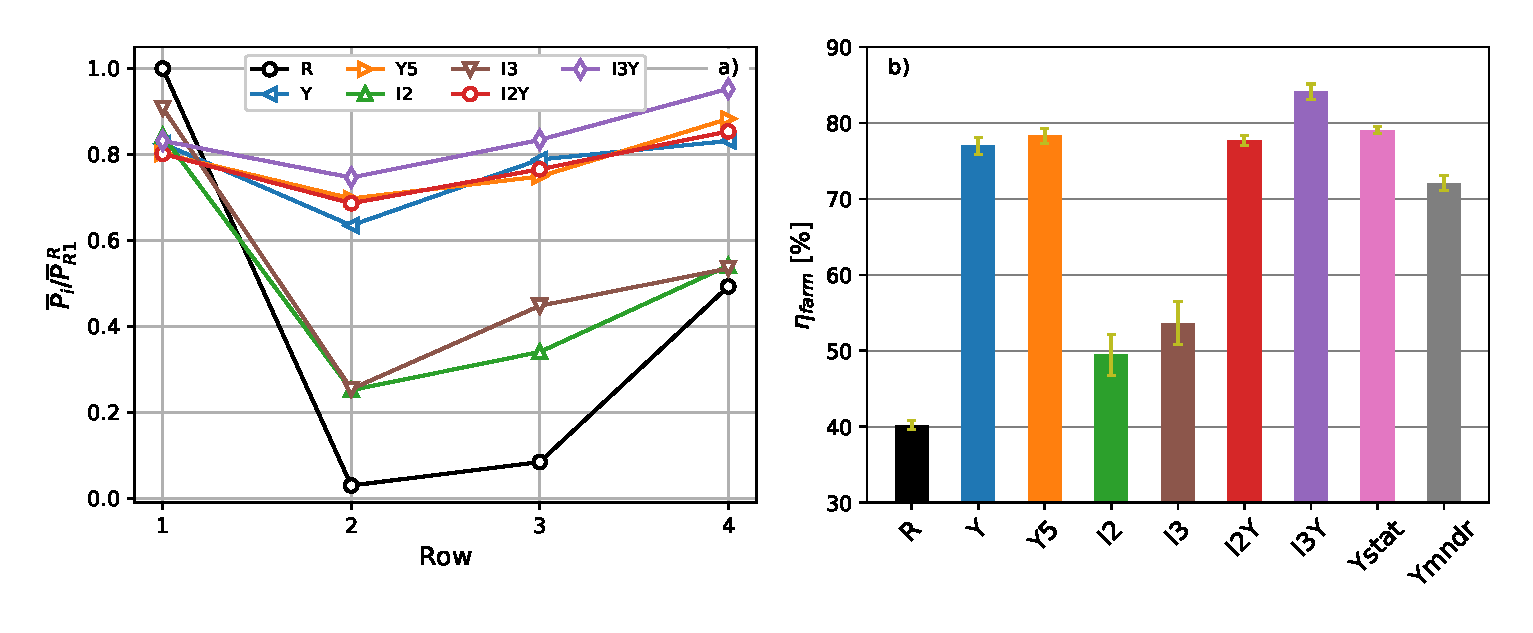
\includegraphics[width=\textwidth]{chapters/optimal_yaw_control/power_row_lam_eff.eps}
		\caption[Wind-farm power extraction and efficiency for uniform inflow.]{Wind-farm power extraction. \emph{a) } Row-averaged power, normalized by first-row power of reference case R. \emph{b) } Wind-farm efficiency $\eta_{\text{farm}}$ compared to situation in which all turbines are first-row turbines of R case. Errorbars indicate confidence intervals of $\pm$ 2 standard deviations and are calculated using the procedure detailed in Appendix~\ref{ch:app_variance}. \label{fig:power_uniform}}
	\end{figure}
	
	\subsubsection{B. Yaw characteristics}
	
	Figure~\ref{fig:dynamic_uniform} illustrates the time evolution of normalized power extraction and yaw angle of the optimal yawing cases (Y, Y5, I2Y, and I3Y), as defined in Table~\ref{tab:case_definition}. 
	The top panels of Figure~\ref{fig:dynamic_uniform} show that, for all optimal yaw cases, power is curtailed to a limited extent in the first row, whereas power in downstream rows is increased significantly after a delay corresponding to the wake advection time.  
	\begin{figure}
	%	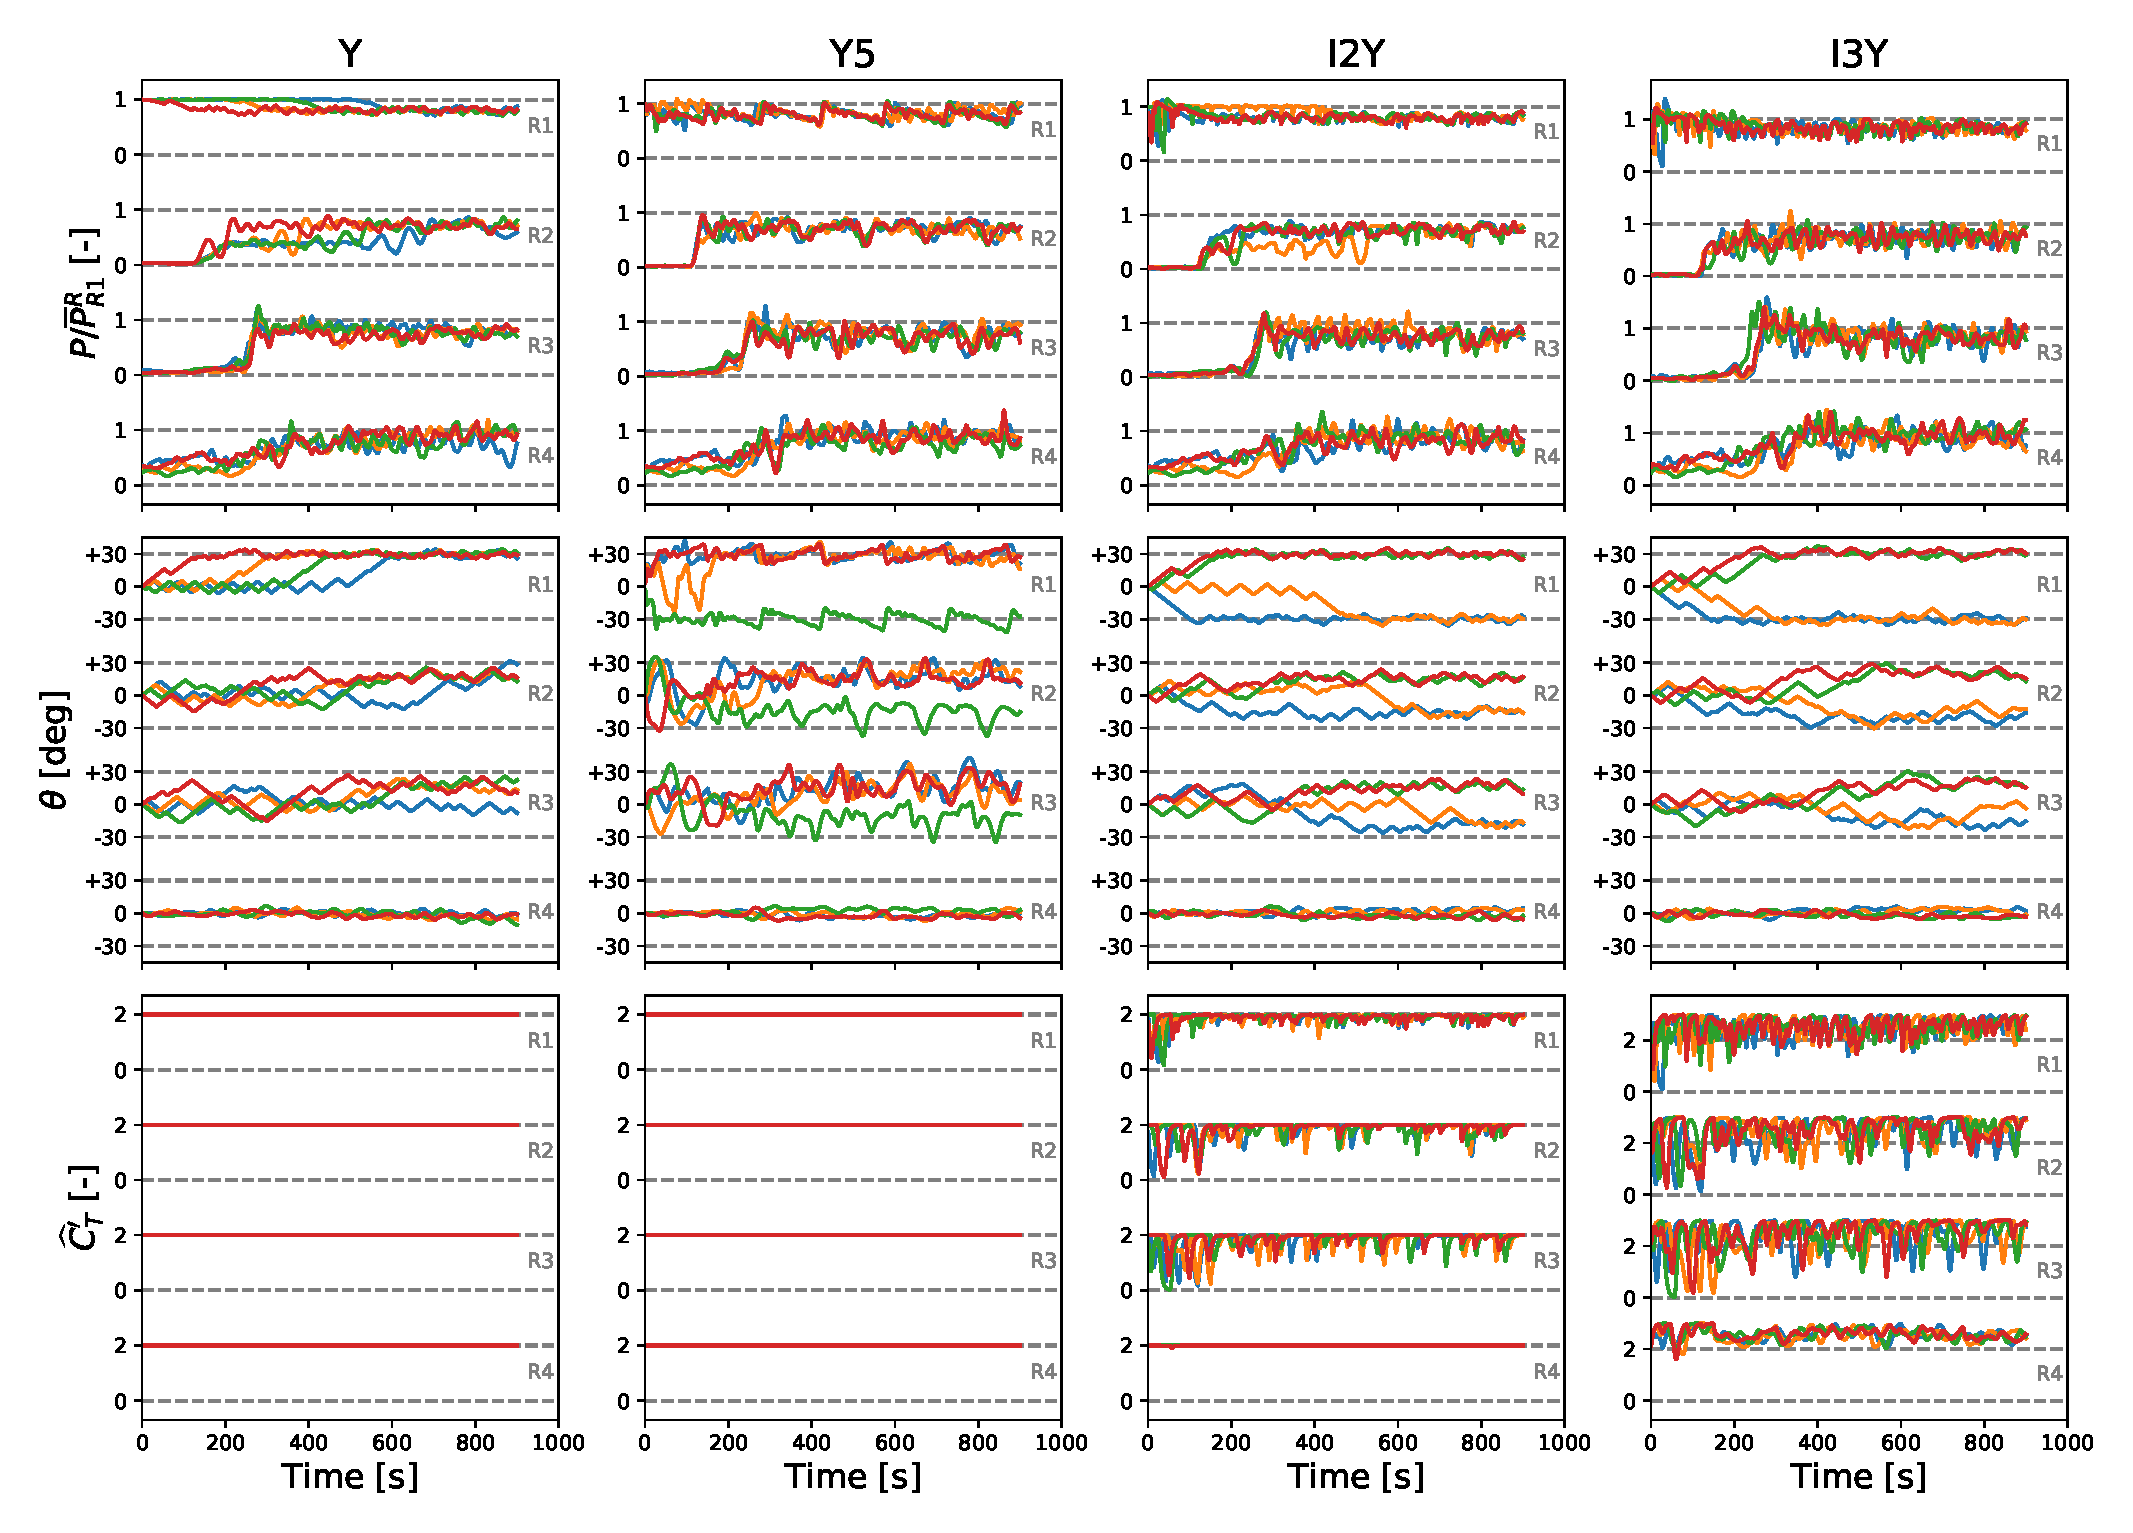
\includegraphics[width=\textwidth]{chapters/optimal_yaw_control/power_angle_ctfilt_lam.eps}
		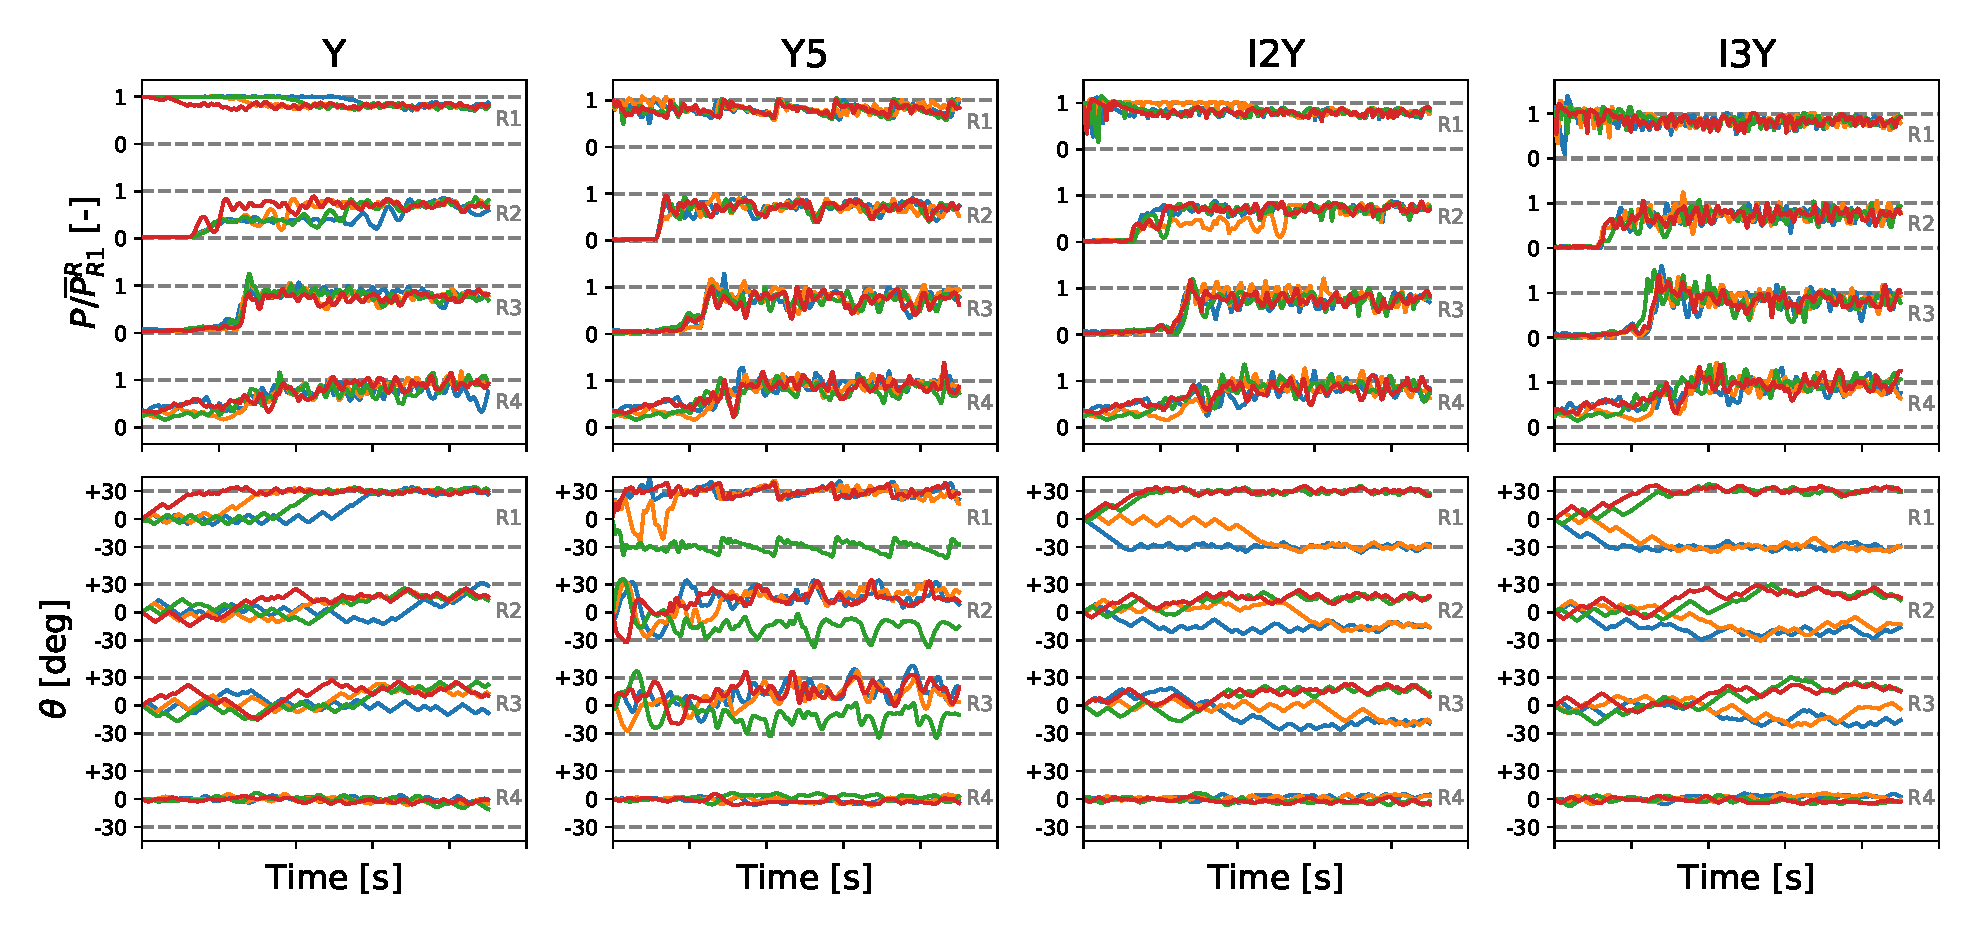
\includegraphics[width=\textwidth]{chapters/optimal_yaw_control/power_yaw_lam.eps}	
		\caption[Time evolution of uniform inflow yaw-enabled cases.]{Time evolution of uniform inflow yaw-enabled cases. \emph{Top: } Turbine power extraction $P$, normalized by mean first row power in the uncontrolled reference $\overline{P}_{R1}^R$. \emph{Bottom: } Yaw angle $\theta$. Line colors indicate different turbine columns as indicated in Figure~\ref{fig:initial_conditions_flow_yaw} ({\color{C1} C1}, {\color{C2} C2}, {\color{C3} C3}, {\color{C4} C4}), i.e. every line represents a single wind turbine. \label{fig:dynamic_uniform}}
	\end{figure}
	
	Turning to the time evolution of the yaw angle $\theta$, a first observation is that, although the 4 columns of the considered wind farm are statistically equivalent in the reference case, their behavior in an optimal control setting is heterogeneous. For example, for case Y, the first-row behavior of the yaw angle $\theta$ seems to exhibit a bifurcation between 2 limit cycles. On the one hand, the first-row turbines in columns C1, C2, and C3 initially oscillate around the flow-aligned yaw angle of $0^\circ$, triggering a \emph{wake meandering} type of motion. Column C4 on the other hand directly turns to a misaligned yaw angle of $30^\circ$, after which it shows some minor high frequency yaw oscillations. As shown in panel Y of Figure~\ref{fig:flowfield_uniform}, the former wake meandering mechanism mainly acts on increased wake spreading in the lateral direction, and enhances recovery by increasing the contact area between the wake and its surroundings. Turbine row 2 and 3 show more complex oscillations, with additional variability in response to the unsteadiness in local flow conditions. In contrast, the first-row yaw misalignment in column C4 creates a more shallow wake which is \emph{redirected} such that it just misses the downstream turbine. Downstream rows 2 and 3 exhibit some minor oscillations around a yaw misalignment angle of $\approx 17^\circ$, causing further yaw redirection downstream. Since there is no further downstream potential for wake mixing or redirection, the final row consistently shows a yaw angle aligned with the mean flow. Similar time evolutions of the yaw angle are observed for column C2 of combined yaw--induction case I2Y. In cases I3Y and Y5, the wake meandering regime seems to be virtually non-existent and wake redirection is dominant, except for the initial stage of the first-row turbine in column C2. In summary, two distinct and relatively simple mechanisms for power increase through yaw control are found: on the one hand a \emph{dynamic} wake meandering regime is identified, and on the other hand a \emph{static} wake redirection regime is observed. These mechanisms are further analyzed below.
	
	\paragraph{Static yaw regime - wake redirection}
	Figure~\ref{fig:cross_section} shows cross sections of the time-averaged axial velocity field from case Y, taken at half a rotor diameter upstream of rows 2, 3, and 4 in column C4, for which turbines directly go to static yaw angles of 30$^\circ$, 17$^\circ$, and 17$^\circ$ for the first, second, and third row respectively (see Figure~\ref{fig:dynamic_uniform}). The figure illustrates that the yaw misalignment of upstream turbines causes the wake to be redirected away from the downstream ones. Moreover, as observed in recent studies, the wake induced by the yaw-misaligned upstream turbines has a curled shape with counter-rotating vortices at its top and bottom \citep{howland2016wake,bastankhah2016experimental}. The current LES-based flow model allows to directly account for this in developing the control strategies, as the wakes are curled just around the downstream turbines, resulting from a trade-off between limiting upstream power loss and redirecting the wakes sufficiently. The static yaw wake redirection regime observed in the optimal control simulations can be mimicked by imposing fixed yaw misalignments corresponding to the aforementioned values. This simplified control case is denoted as Ystat. 
	
	It can be seen from Figure~\ref{fig:power_uniform}b that Ystat yields approximately the same wind-farm efficiency of 79\% as the optimally controlled yawing cases Y and Y5, suggesting that any dynamic effects observed for turbines in the wake redirection regime are of very minor importance. Furthermore, the fact that the expected value of Ystat is slightly higher than that of Y and Y5 can be attributed to the fact that optimizations are not fully converged, finite-horizon effects possibly have a small negative influence on the optimal control cases, and the wake meandering regime that is present in some turbines for the optimal control cases yields slightly lower power than the pure wake redirection of Ystat.
	
	\begin{figure}
		\includegraphics[width=\textwidth]{chapters/optimal_yaw_control/frontview_yaw.eps}
		\caption[Time-averaged cross-sectional views of streamwise velocity $\widetilde{u}_x$ for case Y at a distance $D/2$ upstream of the downstream turbines in column C4.]{Time-averaged cross-sectional views of streamwise velocity $\widetilde{u}_x$ for case Y at a distance $D/2$ upstream of the downstream turbines in column C4. Arrows represent the projection of the velocity vector on the cross-sectional plane. Dashed white lines indicate turbine rotor locations. Coloring is in units of m s$^{-1}$. \label{fig:cross_section}}
	\end{figure}
	
	\paragraph{Dynamic yaw regime - wake meandering}
	Figure~\ref{fig:spec_uniform} shows row-averaged power spectra of the yaw angle $\theta$. We focus on relatively slow dynamics: spectra are shown up to a Strouhal number $St = f D/U_\infty = 0.8$, corresponding to variations with a time period longer than 15 s. The figure shows that, for the upstream rows 1 to 3, the variance of the fast yawing case Y5 is significantly higher than the slow yawing cases Y, I2Y, and I3Y. The first row of case Y shows a significant peak around $St = f D/U_\infty= 0.2$, corresponding to the frequency of the aforementioned oscillations around aligned yaw angles, triggering wake meandering. Smaller subsequent peaks at harmonics of this frequency are also observed. Indeed, a Strouhal number in the range of 0.1 -- 0.3 has been associated with natural wake meandering before in various studies \citep{medici2008measurements, howard2015statistics}. Although attenuated, this peak seems to manifest itself to a limited degree in downstream rows as well. Furthermore, traces of this behavior are also observed for case I2Y, for which it was already mentioned that the first row of column C2 showed behavior consistent with a regime triggering wake meandering. In contrast, as observed qualitatively from Figure~\ref{fig:dynamic_uniform}, cases Y5 and I3Y show no strongly coherent dynamic yaw characteristics, indicating that static wake redirection yaw is dominant here. Similar to the simplified static yaw case derived from the wake redirection behavior in previous paragraph, the wake meandering regime can be approximated by imposing a simple on--off control on the first row turbines, with an alternating yaw rate $\omega = 0.3^\circ$ s$^{-1}$ in both directions with a frequency corresponding to a Strouhal number $St = 0.2$. The coherent dynamics and phase differences of the yaw rates in the downstream turbines are more complex. Therefore, these turbines are not yawed in the derived control case. This simplified case is further denoted as Ymndr. Figure~\ref{fig:power_uniform}b illustrated that, by simply applying this on--off control in the first-row turbine, a wind-farm efficiency of about 72\% can be attained.
	
	\begin{figure}
		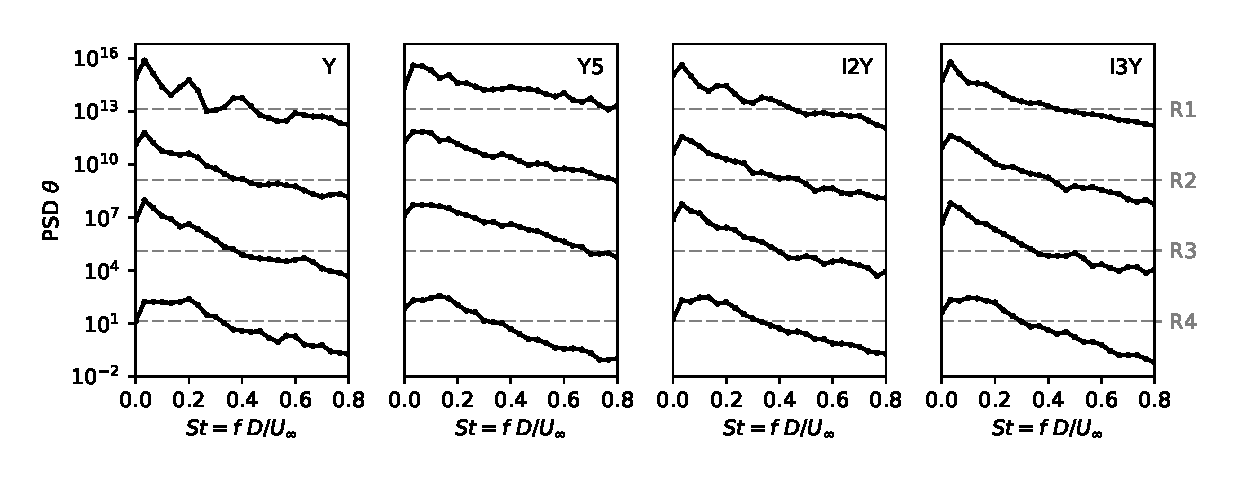
\includegraphics[width=\textwidth]{chapters/optimal_yaw_control/PSD_laminar.eps}
		\caption[Row-averaged power spectral density estimate of yaw angle $\theta$ as a function of Strouhal number $St = f D/U_\infty$.]{Row-averaged power spectral density estimate of yaw angle $\theta$ as a function of Strouhal number $St = f D/U_\infty$. Spectra of different rows are shifted vertically for clarity. Horizontal dashed lines indicate identical reference values for each row.\label{fig:spec_uniform}}
	\end{figure}
	
	
	\subsubsection{C. Induction characteristics}
	Figure~\ref{fig:dynamic_ctfilt} illustrates the time evolution of normalized power extraction and thrust coefficient of the optimal induction cases (I2, I3, I2Y, and I3Y), as defined in Table~\ref{tab:case_definition}. In contrast to the heterogeneous behavior in different columns for the yaw angles as shown in Figure~\ref{fig:dynamic_uniform} above, the induction coefficient behavior is similar for each column, and is illustrated for column C1 only. The top panels of Figure~\ref{fig:dynamic_ctfilt} indicate that, for the exclusively inductive cases I2 and I3, first-row power is pulsed severely, leading to intermittent increases in downstream power extraction. This differs from the combined yaw--induction cases, which show much smoother power extraction dynamics. 
	\begin{figure}
		%	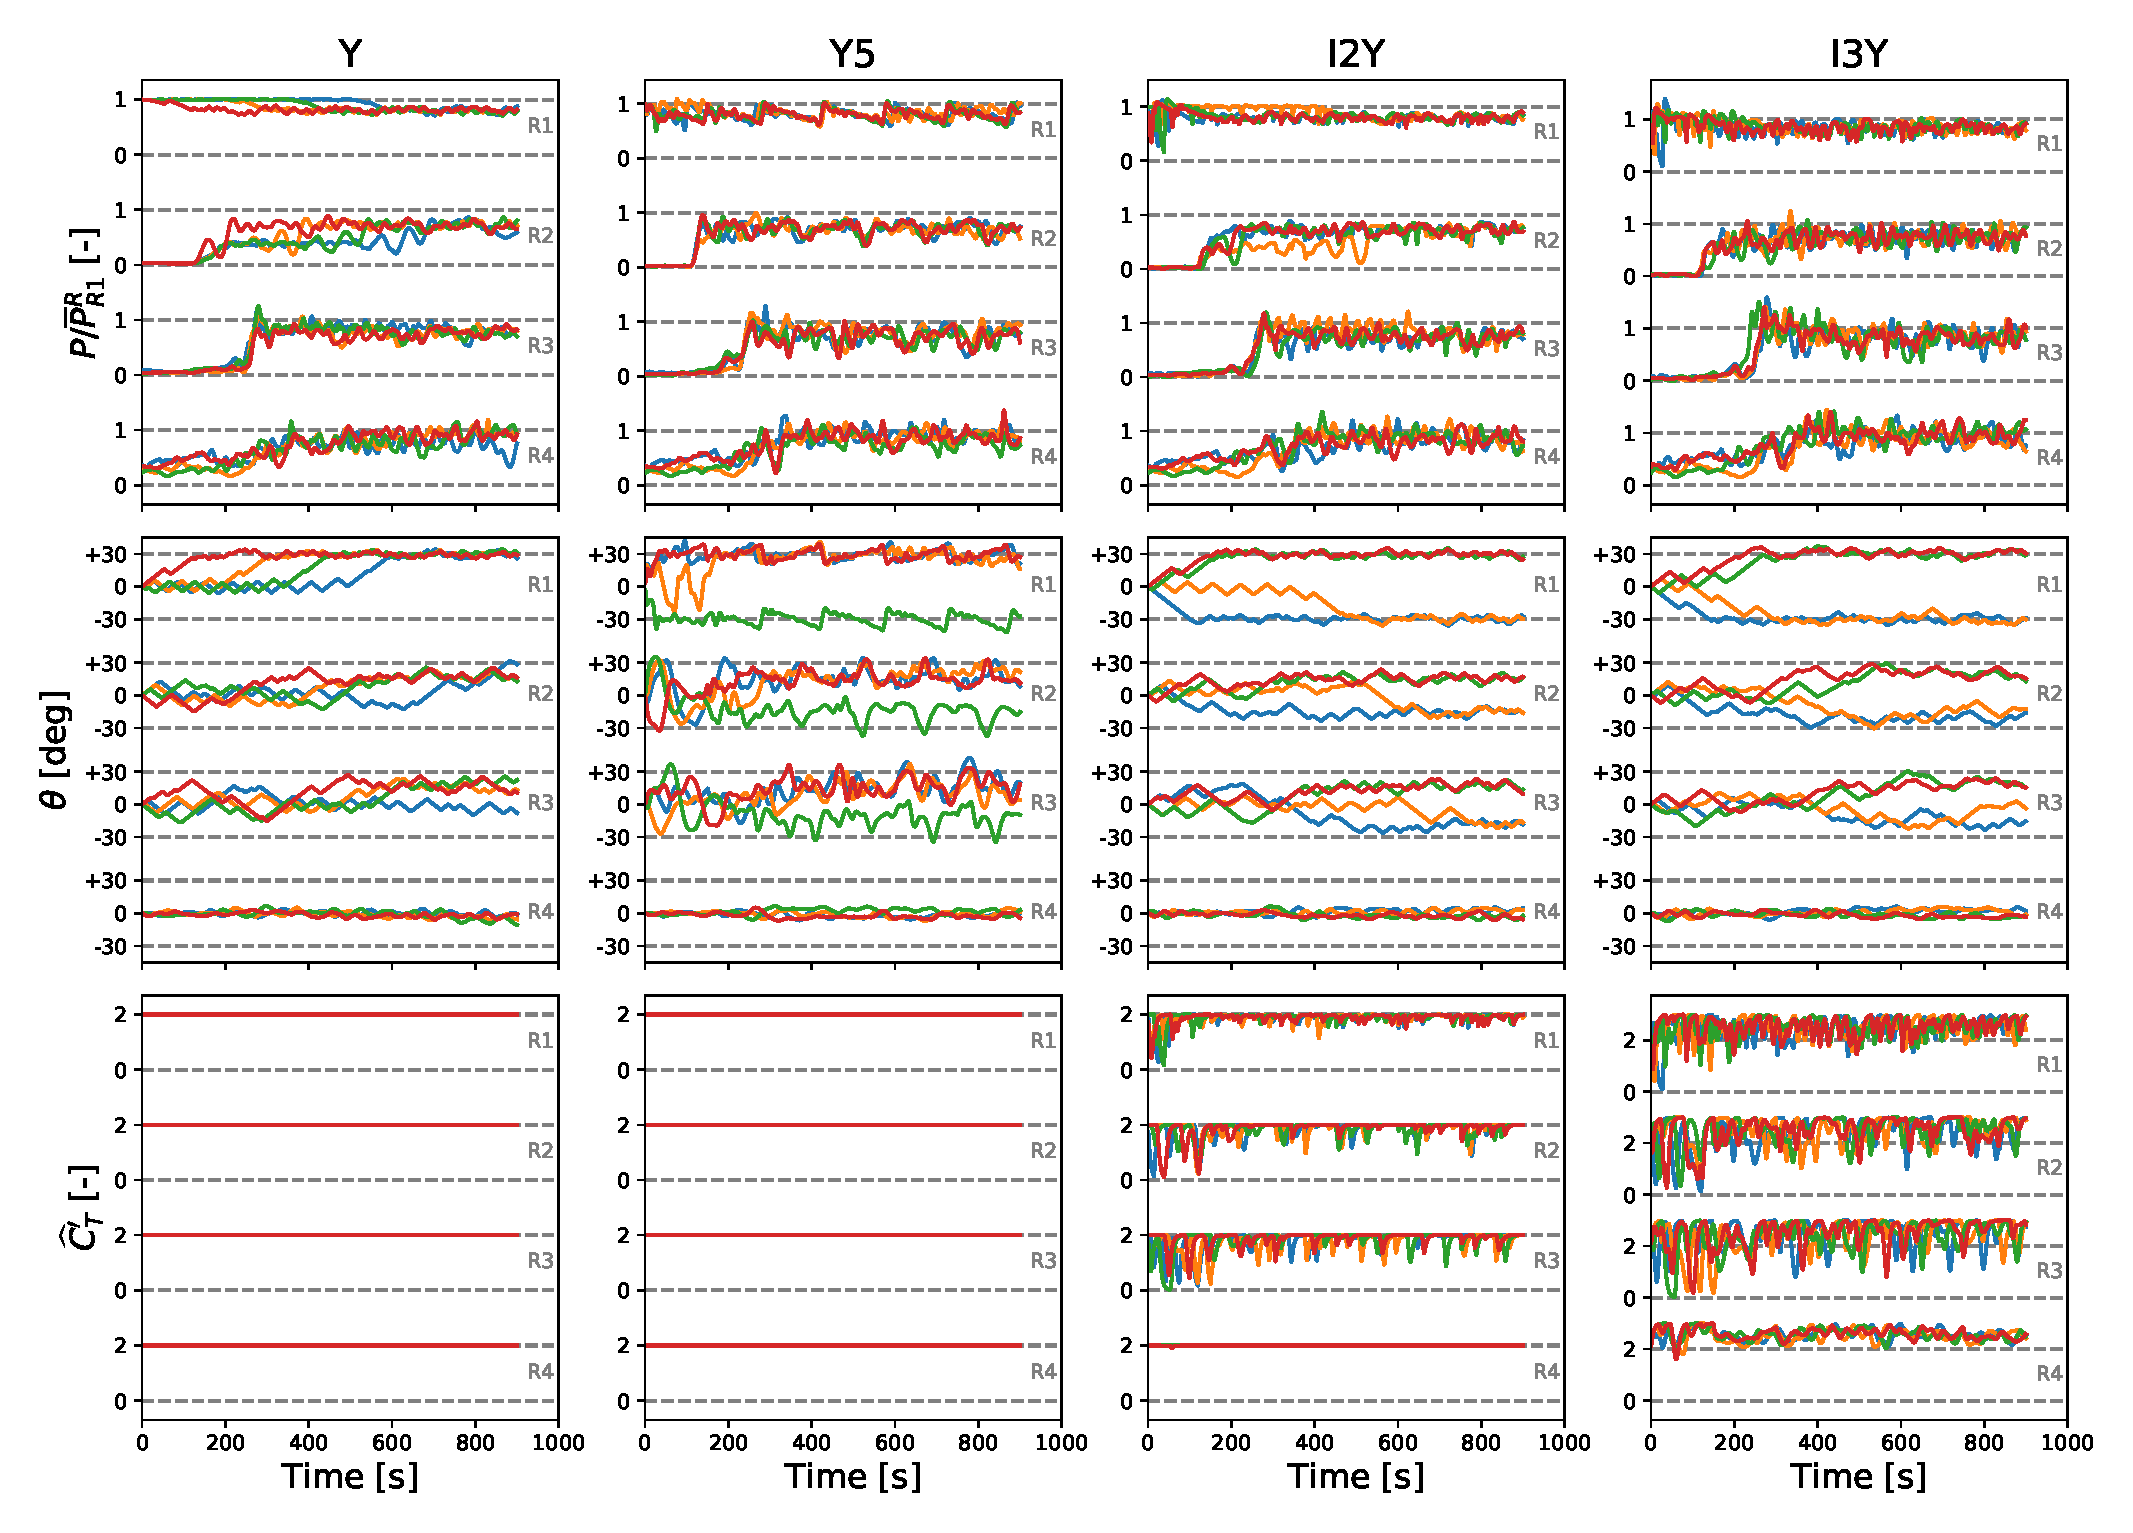
\includegraphics[width=\textwidth]{chapters/optimal_yaw_control/power_angle_ctfilt_lam.eps}
		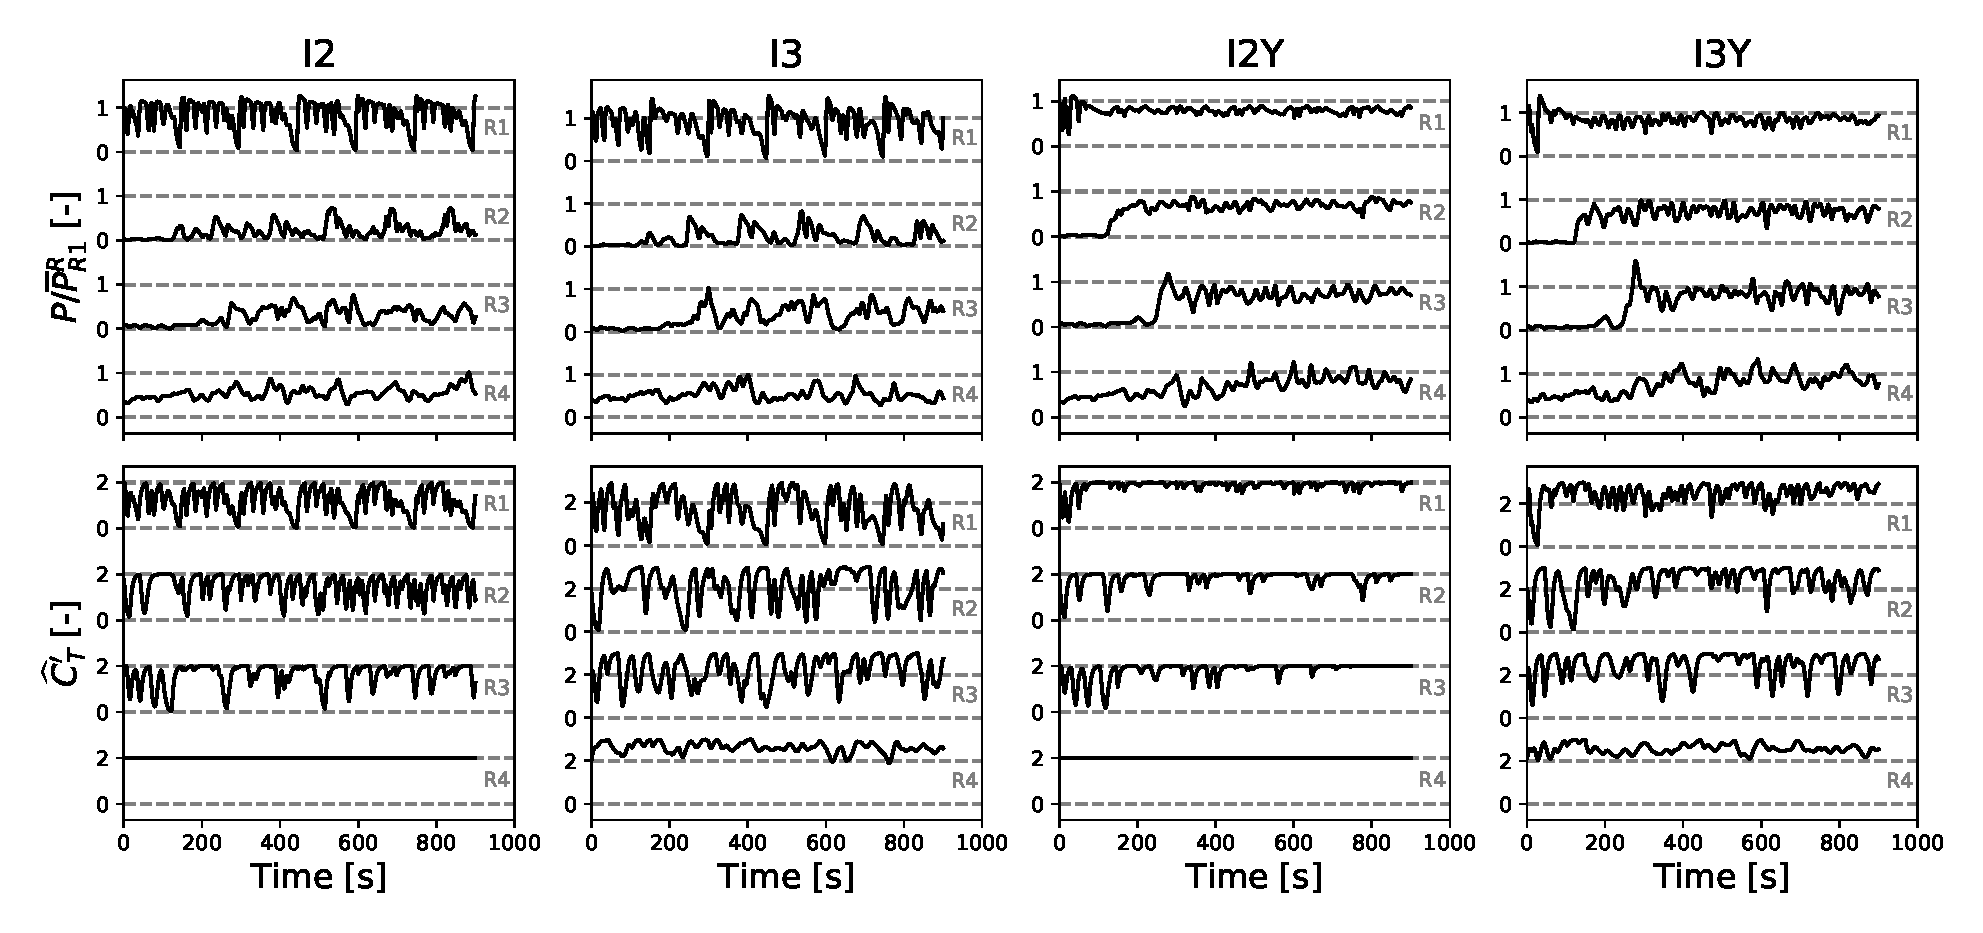
\includegraphics[width=\textwidth]{chapters/optimal_yaw_control/power_ctfilt_lam_bw.eps}	
		\caption[Time evolution of column C1 in uniform inflow induction-enabled cases.]{Time evolution of column C1 in uniform inflow induction-enabled cases. \emph{Top: } Turbine power extraction $P$, normalized by mean first row power in the uncontrolled reference $\overline{P}_{R1}^R$. \emph{Bottom: } Thrust coefficient $\widehat{C}_T'$. \label{fig:dynamic_ctfilt}}
	\end{figure}
	
	Also the thrust coefficient dynamics vary significantly between different cases: the first-row thrust coefficients of I2 and I3 exhibit periodic oscillatory traits, and the downstream rows of these cases show somewhat more chaotic dynamics in response to unsteady flow conditions resulting from upstream actuation. Note that the period associated with this periodicity corresponds to the window length, i.e. 150 s, hence indicating that these cases are reacting to finite-horizon effects. 
	
	The underinductive yawing case I2Y features only minor deviations from the reference upper bound value of $\cthat = 2$, especially for $t > 200$ s. This can be explained based on the fact that, after this time, most turbines are yawed with respect to the incoming flow as shown in Figure~\ref{fig:dynamic_uniform}, resulting in a lower axial velocity $V$, and hence a lower thrust force. Further reduction of this thrust force through lower thrust coefficients seems to show only very limited potential in increasing wind-farm power. 
	
	A converse reasoning can be used to explain the induction characteristics in case I3Y: the higher mean values of $\cthat$ in rows 1, 2, and 3 indicate that the wind farm benefits from compensating for the thrust force reduction in yawed turbines by increasing their axial induction. Note that, for the exclusively overinductive case I3, the mean thrust coefficient in the same rows is slightly lower than 2. The last-row turbines of both overinductive cases (I3 and I3Y) are both aligned with the mean flow and show a similar slight increase in the mean thrust coefficient. 
	
	The current section showed results for the steady uniform inflow cases. All controlled cases increase wind-farm efficiency by a significant amount, with the yaw-enabled cases significantly outperforming cases based on induction control only. Given the current quiescent ambient flow conditions, simple yaw behavior was identified, i.e. dynamic yaw triggering wake meandering on one hand, and steady yaw resulting in wake redirection on the other hand. Moreover, the simplified control cases Ystat and Ymndr derived from this behavior attain similar wind-farm efficiencies as the optimal control cases. In the next section, unsteady and turbulent inflow conditions are applied, and it is investigated whether similar simplified control methods can be applied.

\subsection{Turbulent inflow}\label{sec:opt_yaw_turb}
	Figure~\ref{fig:flowfield_turb} illustrates snapshots of instantaneous streamwise velocity and wall-normal vorticity at hub height at t = 450 s for the reference case R, yawing case Y, overinductive case I3, and combined yaw--overinductive case I3Y. In comparison to the uniform inflow set in Figure~\ref{fig:flowfield_uniform}, the ambient turbulence introduces background vorticity and already destabilizes turbine wakes even in the reference case. Furthermore, wake behavior is much more chaotic and, although traces of wake redirection can be observed for cases Y and I3Y, differences between the flow fields of different cases are far less obvious than in uniform inflow. 
	\begin{figure}
		\includegraphics[width=\textwidth]{chapters/optimal_yaw_control/flow_field_turb.eps}
		\caption[Instantaneous planviews at hub height for turbulent inflow cases at $t= 450$ s.]{Instantaneous planviews at hub height for turbulent inflow cases at $t= 450$ s. \emph{Top: } Streamwise velocity. \emph{Bottom: } Wall-normal vorticity. Coloring is in units of m s$^{-1}$, s$^{-1}$. \label{fig:flowfield_turb}}
	\end{figure}
	
	Similar to the presentation of uniform inflow results in the previous section, firstly power extraction and wind-farm efficiency are illustrated, after which the induction characteristics of inductive cases are shown. Finally, the yaw and power characteristics of the yaw-enabled control cases are described.
	
	\subsubsection{A. Power extraction and wind-farm efficiency}
	Figure~\ref{fig:power_turb} depicts time-averaged wind-farm power results in the same manner as Figure~\ref{fig:power_uniform}. Figure~\ref{fig:power_turb}a illustrates the row-averaged power extraction for the reference and optimal control cases. Note firstly the much higher power extraction in rows 2 and 3 for the reference case than in the uniform set, caused by the natural destabilization and mixing of turbine wakes by the ambient turbulence. Further, the figure shows that first-row power is being curtailed in all controlled cases. However, for the inductive cases I2 and I3, this curtailment is limited to below 5\%. Significant power gains are achieved in all downstream rows of the inductive cases, except for the second row of I2. For the yaw-enabled cases, curtailment in the first row is smaller than in the uniform inflow set at around 15\%, yet similar flattened power profiles are obtained. 
	
	Figure~\ref{fig:power_turb}b illustrates the wind-farm efficiency for the reference case and the optimal control cases. Similar to the set of uniform inflow cases, also for turbulent inflow two simplified control cases Ystat and Ymndr are defined. These cases are further described and discussed below. A first observation is the higher reference efficiency at 58\% compared to the uniform inflow value of 40\%. Further, the power variability has increased in all cases, as indicated by the wider confidence intervals of the expected values (procedure for calculation of confidence intervals further detailed in Appendix~\ref{ch:app_variance}). The exclusively inductive cases I2 and I3 achieve wind-farm efficiencies of 63\% and 67\% respectively. The optimal yaw cases Y, Y5, I2Y, and I3Y attain slightly higher efficiencies of 70\%, 75\%, 73\%, and 78\% respectively. Note that, for unsteady ambient flow conditions, the faster yaw rate in case Y5 significantly increases the efficiency over the standard yaw case Y. The addition of underinduction control (I2Y) provides a small benefit over standard yaw control (Y), but the highest efficiency is again achieved by overinductive yaw control (I3Y). 
	
	\begin{figure}
		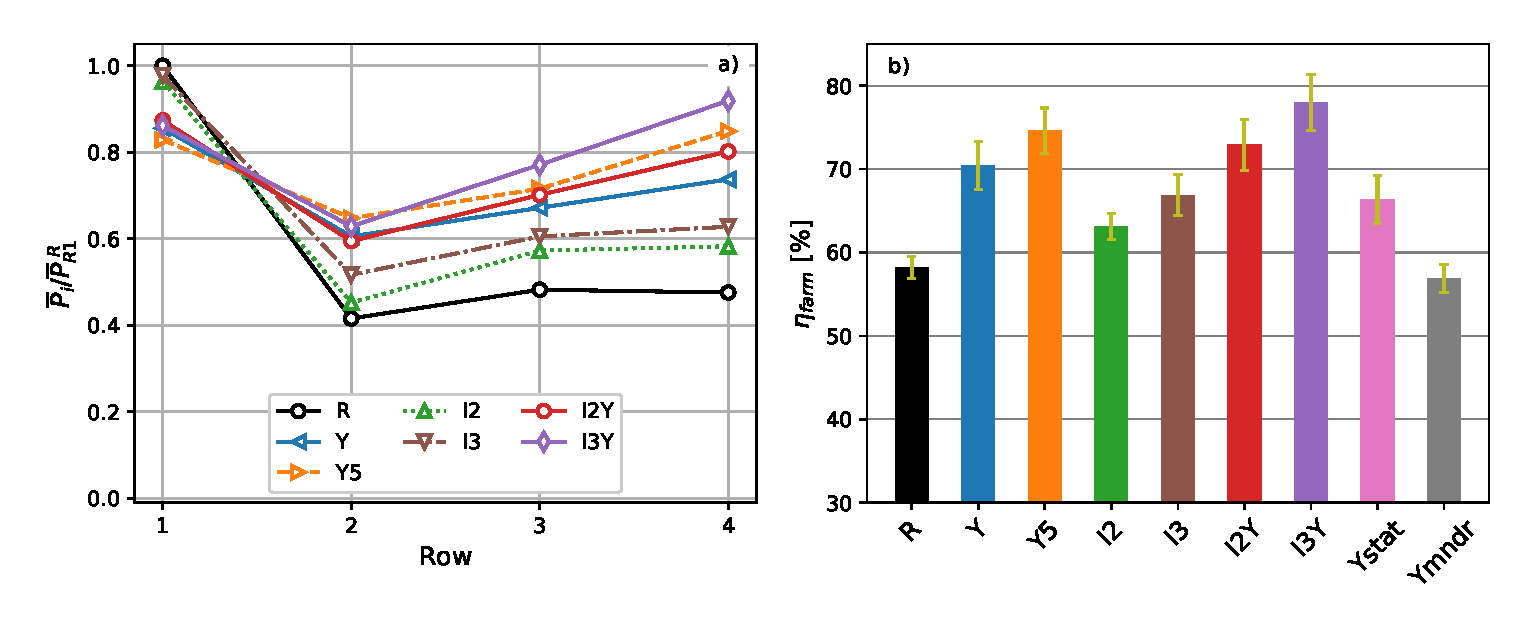
\includegraphics[width=\textwidth]{chapters/optimal_yaw_control/power_row_turb_eff.eps}
		\caption[Wind-farm power extraction for turbulent inflow.]{Wind-farm power extraction. \emph{a) } Column-averaged power per row, normalized by first-row power of reference case R. \emph{b) } Wind-farm efficiency $\eta_{\text{farm}}$ compared to situation in which all turbines are first-row turbines of R case. Errorbars indicate confidence intervals of $\pm$ 2 standard deviations and are calculated using the procedure detailed in Appendix~\ref{ch:app_variance}. \label{fig:power_turb}}
	\end{figure}
	
	\subsubsection{B. Yaw characteristics}
	 Figure~\ref{fig:dynamic_turb} indicates that both power and yaw angle exhibit significantly more variability compared to the uniform inflow set for all cases. Since wake meandering is already naturally triggered in turbulent boundary layers, the typical wake meandering regime with oscillations around yaw-aligned conditions is not directly observed qualitatively for any of the cases here. In contrast, the yaw-enabled cases all seem to turn to the wake redirection regime, characterized by approximately the same yaw angles as in the uniform inflow cases. Note however that there is significant response of the yaw angle to background variability in local flow conditions for all cases, even causing the yaw angle to flip signs temporarily. 
	\begin{figure}
		%	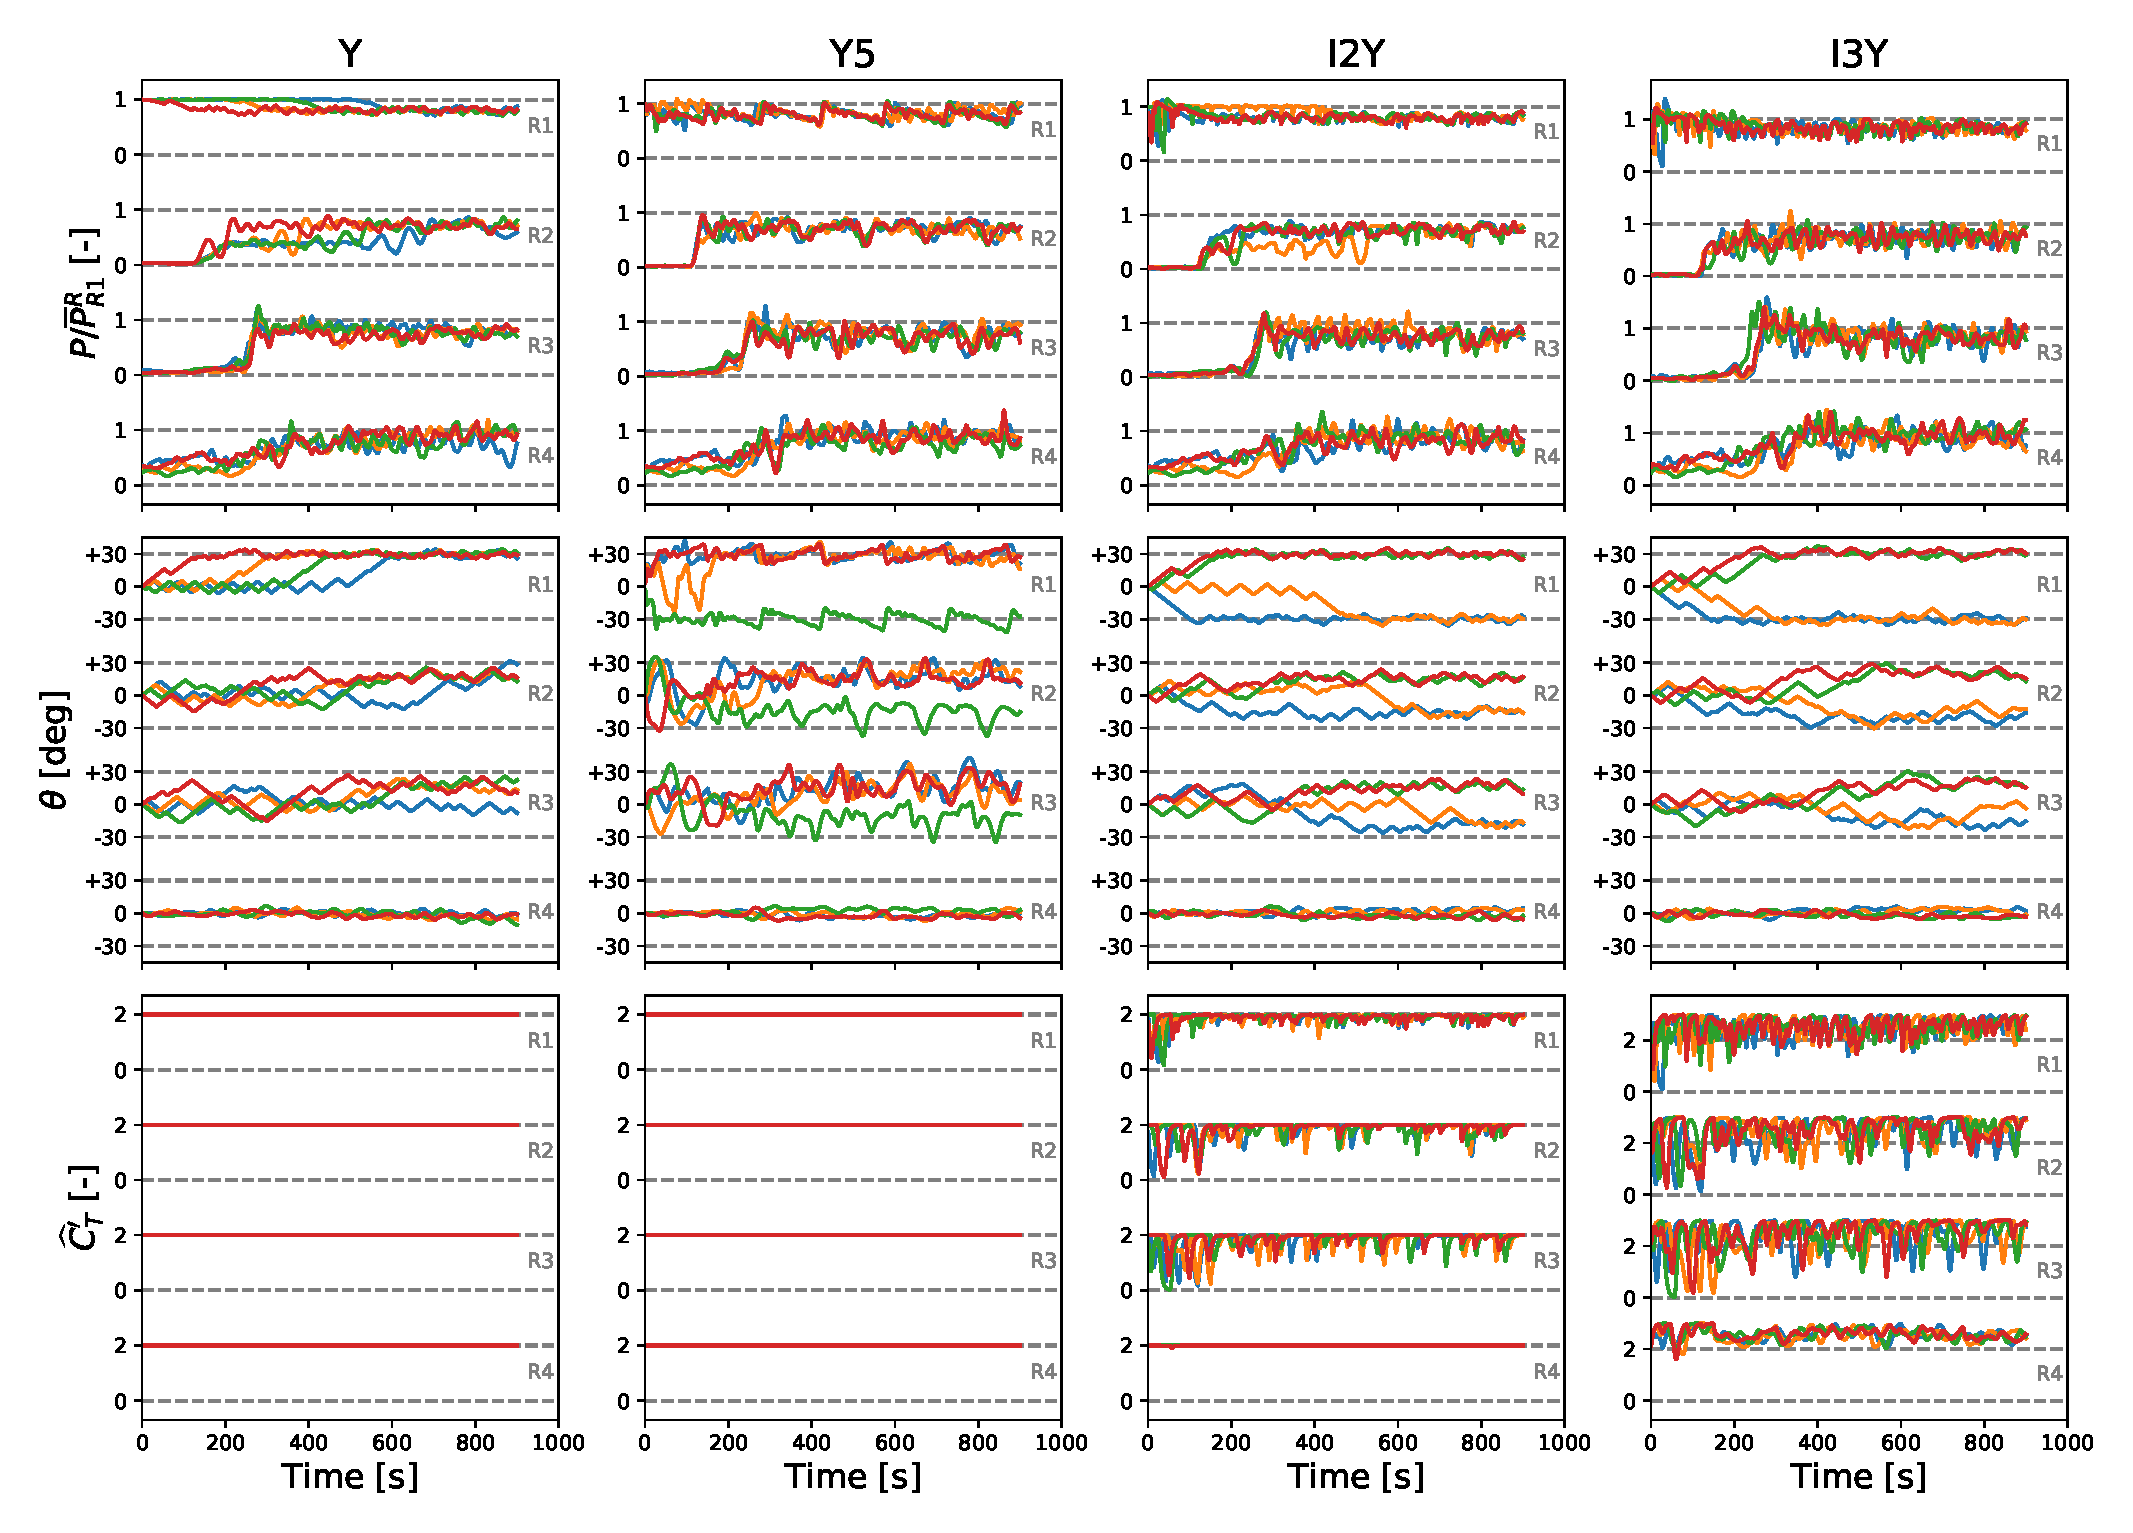
\includegraphics[width=\textwidth]{chapters/optimal_yaw_control/power_angle_ctfilt_lam.eps}
		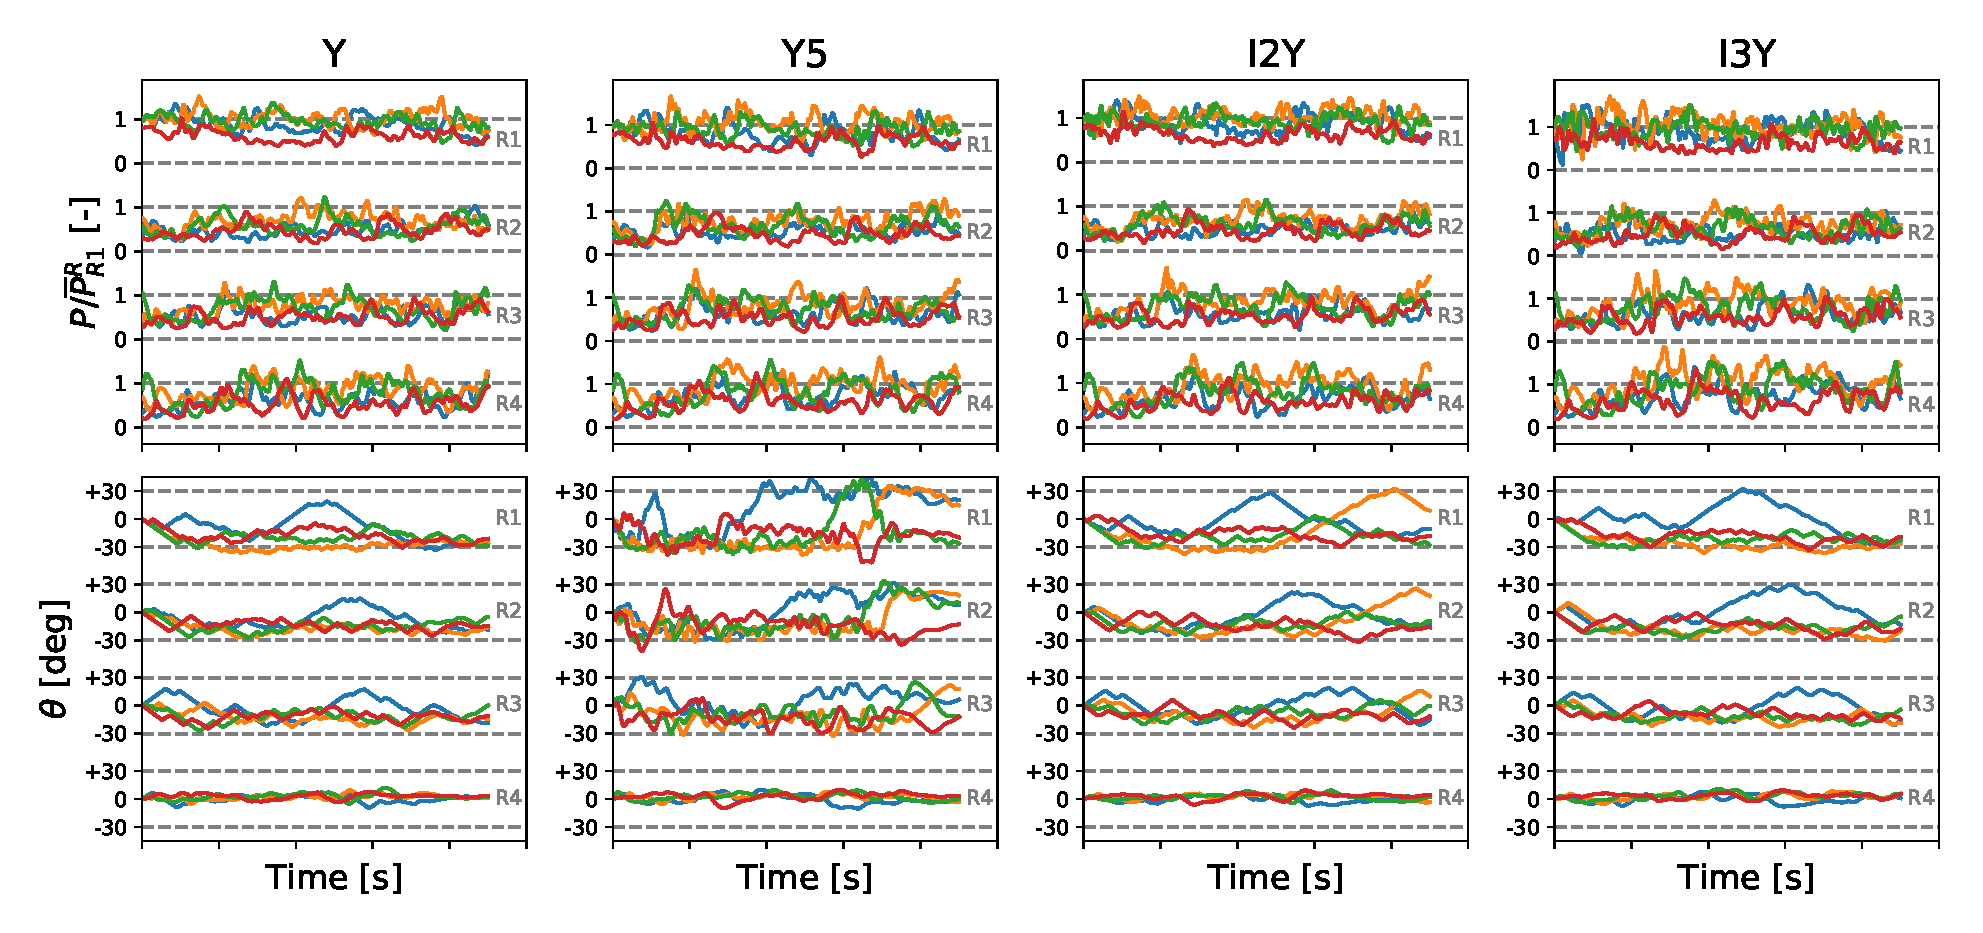
\includegraphics[width=\textwidth]{chapters/optimal_yaw_control/power_yaw_turb.eps}	
		\caption[Time evolution of turbulent inflow yaw-enabled cases.]{Time evolution of turbulent inflow yaw-enabled cases. \emph{Top: } Turbine power extraction $P$, normalized by mean first row power in the uncontrolled reference $\overline{P}_{R1}^R$. \emph{Bottom: } Yaw angle $\theta$. Line colors indicate different turbine columns as indicated in Figure~\ref{fig:initial_conditions_flow_yaw} ({\color{C1} C1}, {\color{C2} C2}, {\color{C3} C3}, {\color{C4} C4}), i.e. every line represents a single wind turbine. \label{fig:dynamic_turb}}
	\end{figure}

	Figure~\ref{fig:cross_section_turb} illustrates time-averaged cross sections of streamwise velocity just upstream of the column C4 turbines for reference case R and yawing case Y. Although wake redirection is complicated by the unsteady inflow, similar deflected and curl-shaped wakes with counter-rotating vortex pairs can be observed for case Y, albeit less explicit than in uniform inflow. Similar characteristics were observed for the other yawing cases Y5, I2Y, and I3Y (not further shown here). Given this information, a similar simplified steady yaw redirection case Ystat was defined, based on the same yaw angles as in the uniform inflow set, i.e. 30$^\circ$, 17$^\circ$, and 17$^\circ$ in rows 1, 2, and 3 respectively. Figure~\ref{fig:power_turb}b illustrates that, although steady yaw control succesfully increases wind-farm efficiency to 66\%, this value is surpassed significantly by the dynamic yawing cases presented above.
	\begin{figure}
		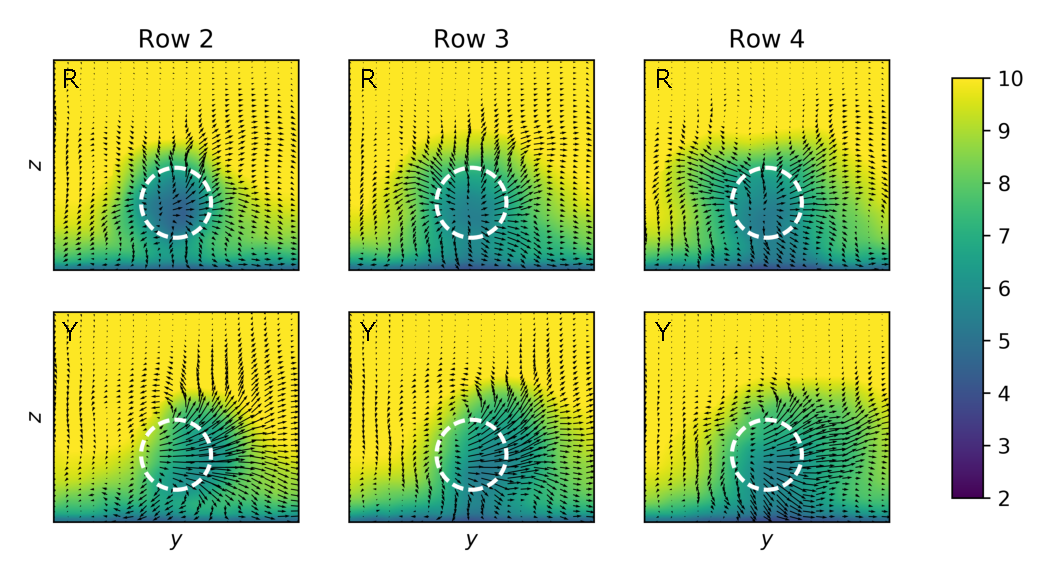
\includegraphics[width=\textwidth]{chapters/optimal_yaw_control/frontview_yaw_turb.eps}
		\caption[Time-averaged cross-sectional views of streamwise velocity $\widetilde{u}_x$ at a distance $D/2$ upstream of the downstream turbines in column C4.]{Time-averaged cross-sectional views of streamwise velocity $\widetilde{u}_x$ at a distance $D/2$ upstream of the downstream turbines in column C4. Arrows represent the projection of the velocity vector on the cross-sectional plane. Dashed white lines indicate turbine rotor locations. Coloring is in units of m s$^{-1}$. \label{fig:cross_section_turb}}
	\end{figure}

	Figure~\ref{fig:spec_turbulent} shows power spectral densities of the yaw angle $\theta$. Although much less apparent than in the uniform inflow, faint local increases in some of the spectra around $St = 0.2$ can be seen. This raises the suspicion that also in the turbulent inflow case, for which wake meandering is already triggered naturally, the optimizer possibly reinforces meandering through yaw actuation in this frequency range. Therefore, an identical meandering case Ymndr, with on--off yaw control at a rate of $\omega = 0.3^\circ$ s$^{-1}$ in the first row was defined. However, Figure~\ref{fig:power_turb}b indicates that this strategy does not lead to an increase in wind-farm efficiency. 
	\begin{figure}
		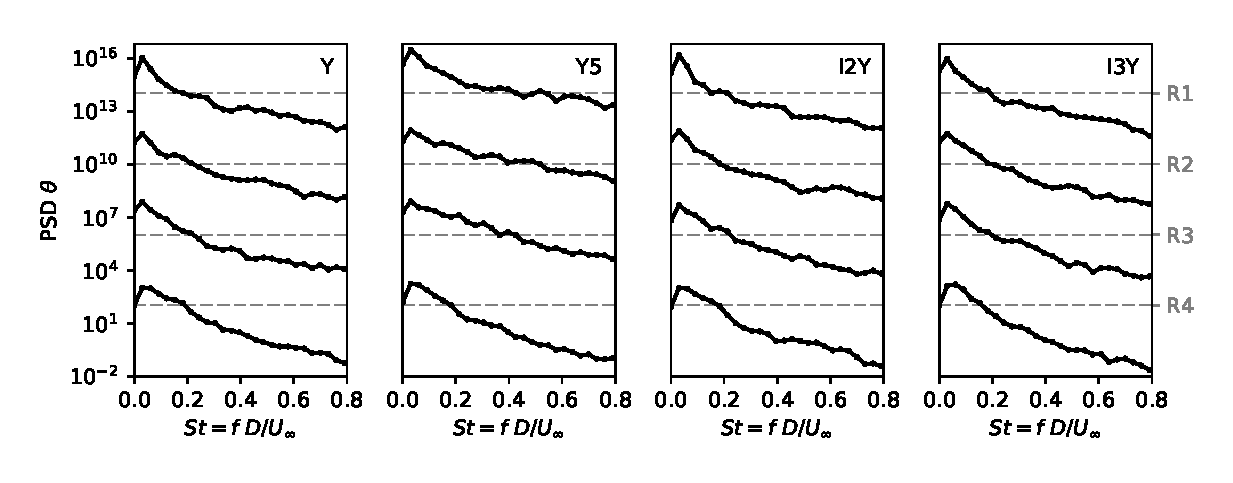
\includegraphics[width=\textwidth]{chapters/optimal_yaw_control/PSD_turbulent.eps}
		\caption[Row-averaged power spectral density estimate of yaw angle $\theta$ as a function of Strouhal number $St = f D/U_\infty$.]{Row-averaged power spectral density estimate of yaw angle $\theta$ as a function of Strouhal number $St = f D/U_\infty$. Spectra of different rows are shifted vertically for clarity. Horizontal dashed lines indicate identical reference values for each row.\label{fig:spec_turbulent}}
	\end{figure}
	
	\subsubsection{C. Induction characteristics}
	Figure~\ref{fig:dynamic_ctfilt_turb} depicts the time evolution of power and induction coefficient for the inductive cases I2, I3, I2Y, and I3Y. Similar to the yaw angles described above, also the thrust coefficient appears much more chaotic than in the uniform inflow set, and shows no visually apparent signs of periodic repetitions in control signals. The underinductive cases I2 and I2Y show little deviation from the upper bound. The overinductive cases show similar behavior to the uniform inflow set, i.e. variations around the reference value of $\cthat = 2$ for I3, and a slight increase in mean thrust coefficient for I3Y. 
	\begin{figure}
		%	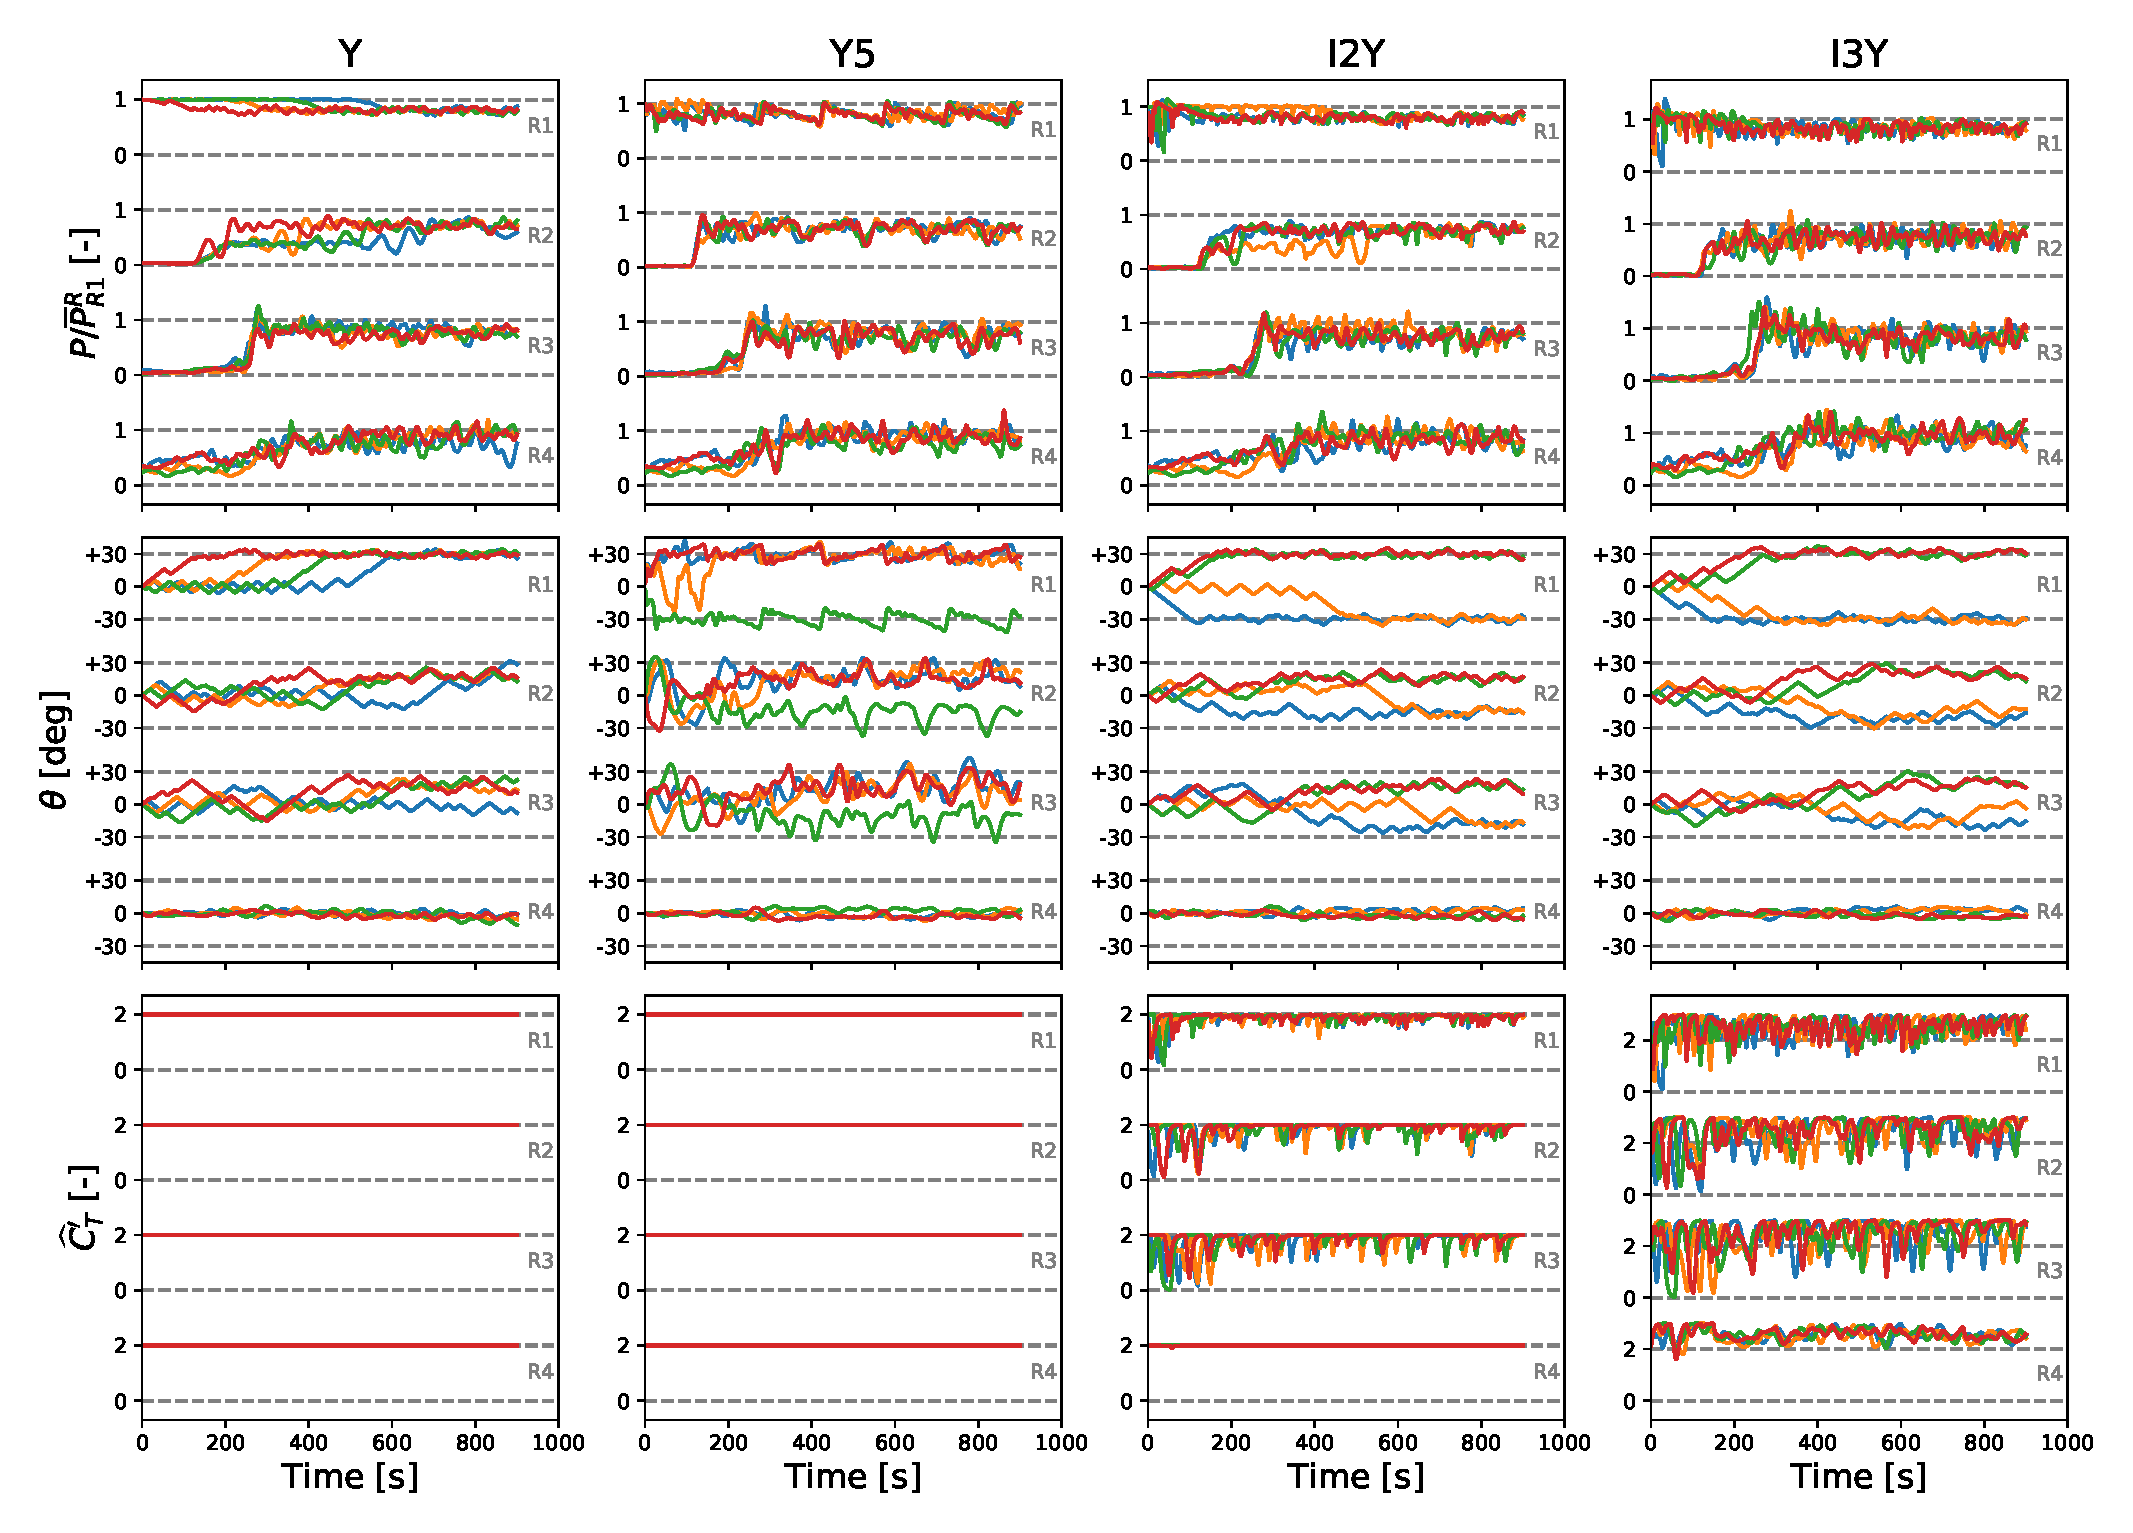
\includegraphics[width=\textwidth]{chapters/optimal_yaw_control/power_angle_ctfilt_lam.eps}
		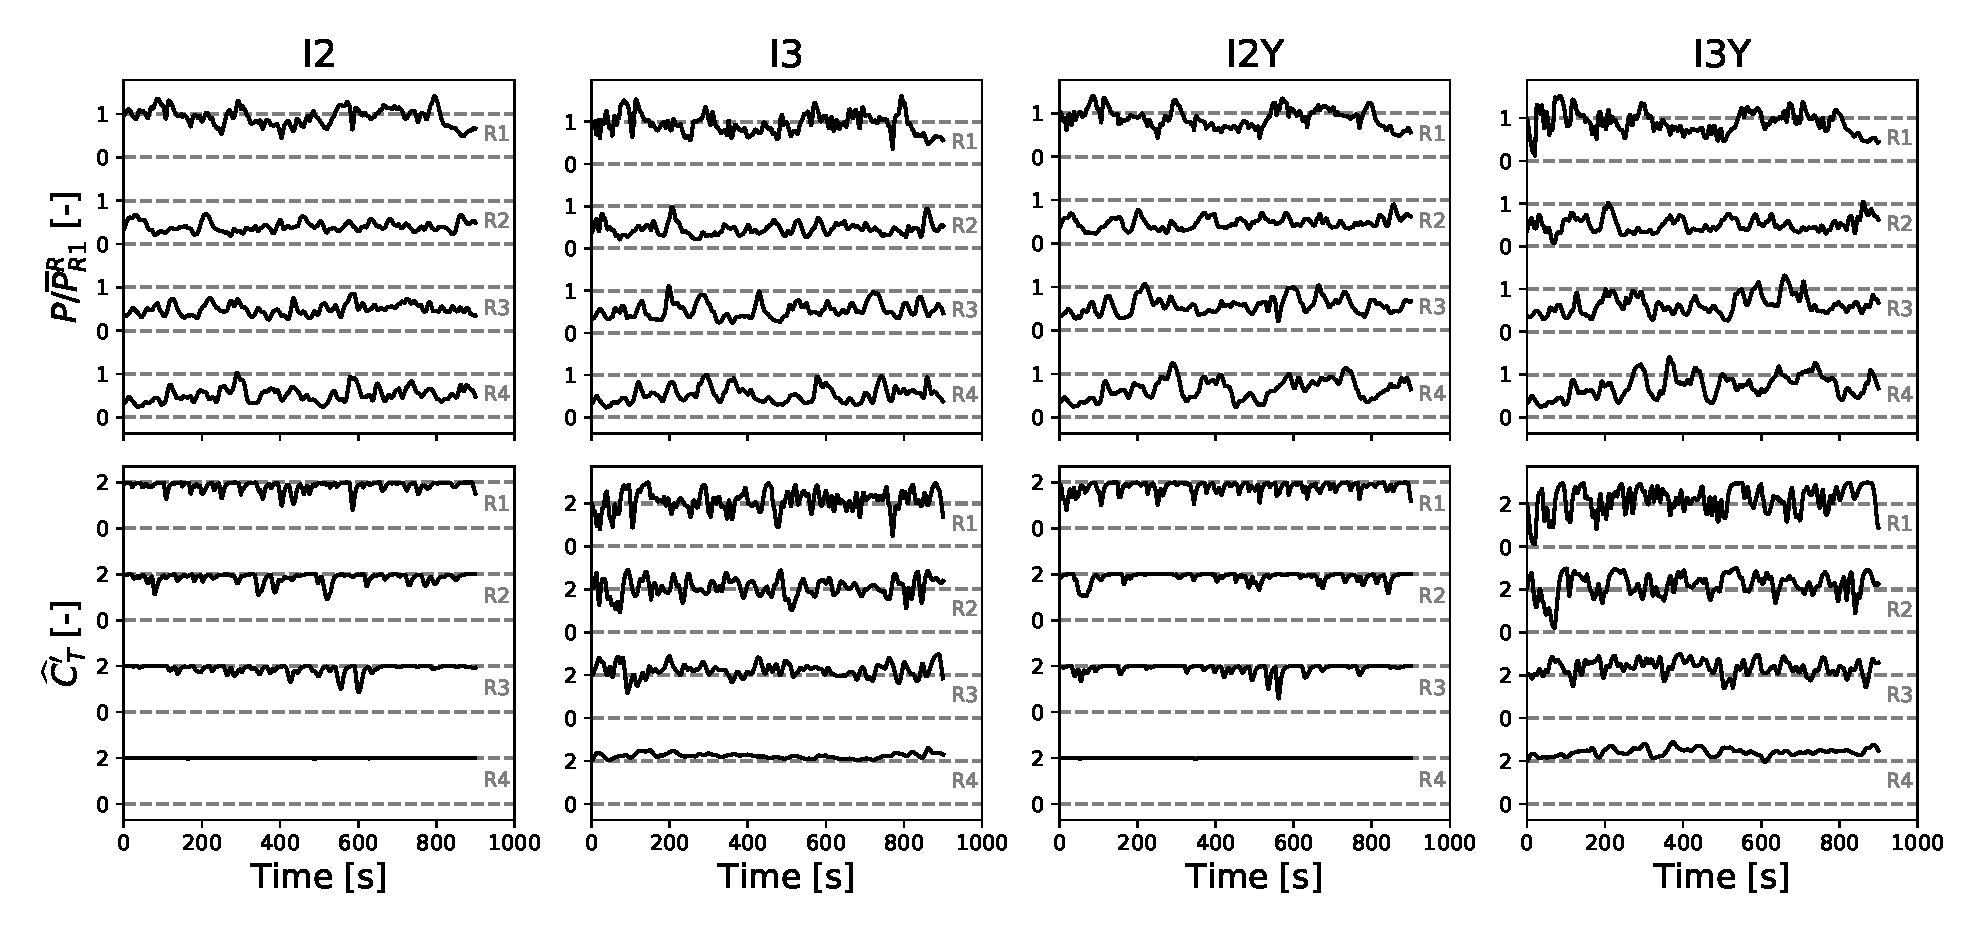
\includegraphics[width=\textwidth]{chapters/optimal_yaw_control/power_ctfilt_turb_bw.eps}	
		\caption[Time evolution of column C1 in turbulent inflow induction-enabled cases.]{Time evolution of column C1 in turbulent inflow induction-enabled cases. \emph{Top: } Turbine power extraction $P$, normalized by mean first row power in the uncontrolled reference $\overline{P}_{R1}^R$. \emph{Bottom: } Thrust coefficient $\widehat{C}_T'$. \label{fig:dynamic_ctfilt_turb}}
	\end{figure}
	



\subsection{Discussion}\label{sec:opt_yaw_disc}
\begin{table}
	\caption{Summary of wind-farm efficiencies and power gains. Optimal control cases are sorted based on farm efficiency. \label{tab:yaw_summary}}
	\centering
	\begin{tabular}{rlll}
		\hline
		&   	 & $\eta_{\text{farm}}^{\text{uniform}}$  & $\eta_{\text{farm}}^{\text{turbulent}}$ \mystrut \mystrut\\
		\hline
		\\
		\multicolumn{1}{l}{\textbf{Greedy control}} & & & \\
		\mystrut		
		Reference   		    	& R 	 & 0.40					       & 0.58\\
		\\
		\hdashline
		\\
		\multicolumn{1}{l}{\textbf{Optimal control}} & & & \\
		\mystrut
		Underinduction  			& I2 	 & 0.49	[+23\%]				   & 0.63 [+8\%]\\
		\mystrut	
		
		Overinduction 	  			& I3 	 & 0.53	[+34\%]				   & 0.67 [+15\%]\\
		\mystrut
		
		Yaw 			    		& Y 	 & 0.77	[+92\%]				   & 0.70 [+21\%]\\
		\mystrut
		
		Underinduction + yaw 		& I2Y 	 & 0.77  [+93\%] 			   & 0.73 [+25\%]\\
		\mystrut
		
		Fast yaw  					& Y5	 & 0.78 [+95\%]  			   & 0.75 [+28\%]\\
		\mystrut
		
		Overinduction + yaw  		& I3Y 	 & 0.84	[+110\%]			   & 0.78 [+34\%]\\
		
		\\
		\hdashline
		\\		
		\multicolumn{1}{l}{\textbf{Simplified control}} & & & \\	
		\mystrut	
		Steady yaw  				& Ystat  & 0.79 	[+97\%]				   & 0.66 [+14\%]\\		        
		\mystrut
		
		Meandering yaw 				& Ymndr  & 0.72 [+79\%] 			   & 0.57 [--2\%]\\					
		\\				
		\hline
	\end{tabular}
\end{table}


Table~\ref{tab:yaw_summary} provides an overview of the efficiencies and power gains attained by each of the control cases described in the previous sections. From the table it can be seen that the relative order, based on wind-farm efficiency, is the same for turbulent and uniform inflow conditions. For cases based on exclusively induction control, i.e. I2 and I3, it can be seen that, although the \emph{relative} increase is larger for uniform inflow, the overall attainable wind-farm efficiency is higher for turbulent inflow conditions. 

\pagebreak

Further results show that, for the current setup, all yaw-enabled cases consistently outperform cases based solely on axial induction control. However, the gap between both is significantly larger for uniform inflow than for turbulent inflow. The main reason for this is that the yawing cases perform better in the absence of inflow turbulence due to the fact that a steady flow allows wakes to be redirected more easily. 

The benefits of combining underinductive axial induction control with yaw control (I2Y) are relatively small: as shown in Figures~\ref{fig:dynamic_uniform} and~\ref{fig:dynamic_turb}, thrust coefficients are barely reduced from their initial upper bound since the thrust forces exerted by turbines in yaw are already reduced through smaller axial velocity components. In contrast, combining overinductive axial induction control with yaw (I3Y) holds much greater promise: in addition to an increase in the mean thrust coefficients, also dynamic thrust variations are observed in Figures~\ref{fig:dynamic_ctfilt} and~\ref{fig:dynamic_ctfilt_turb}, resulting in the highest efficiencies obtained for all cases. 

Based on the time evolution of yaw angles in Figures~\ref{fig:dynamic_uniform} and~\ref{fig:dynamic_turb} two simplified cases were derived. On the one hand a static yaw control case (Ystat) was defined, which steadily deflects wakes away from downstream turbines by imposing yaw misalignments of $30^\circ$, $17^\circ$, and $17^\circ$ in rows 1, 2, and 3 respectively. On the other hand a dynamic yaw control case (Ymndr) was defined, in which an alternating yaw control in the first-row turbine resulting in minor but unsteady yaw misalignments was imposed to reinforce downstream meandering of the wake. It is important to stress that these are control strategies derived from observations in the optimal control simulations, but no optimization was employed upon generating their control signals. 

The yaw angles used in Ystat, as derived from the dynamic cases, are the same for both uniform and turbulent inflow. This indicates that the misalignment angles for steady yaw control are determined by the wind-farm layout geometry, and the dependence on flow conditions is minor. Although Ystat attains virtually identical efficiencies as the dynamic yaw cases Y and Y5 under uniform inflow, its performance under unsteady turbulent flow conditions is surpassed significantly by the latter dynamic cases. This suggests that, in turbulent flows, yaw dynamics play a significant role in increasing wind-farm power in response to continuously changing flow conditions and incident flow angles. This claim is supported by the observation that case Y5 significantly outperforms case Y for turbulent inflow, where this is not the case for uniform inflow. 

Further, simplified case Ymndr succeeds in significantly increasing wind-farm efficiency under uniform inflow, and even surpasses the optimization-based induction cases I2 and I3. This is a remarkable result for this very simple control strategy in which active turbines in the first row perform a simple flapping motion, whereas downstream turbines remain passive as in the reference case. However, in turbulent inflow conditions the same strategy did not lead to an increase in power extraction. This can be explained by the fact that meandering is already triggered naturally in turbulent boundary layers. Instead of actively reinforcing downstream wake meandering, the faint traces of spectral peaks at $St = 0.2$ observed in Figure~\ref{fig:spec_turbulent} might therefore simply be the response of yawing turbines to variability in the incident flow angle induced by natural upstream wake meandering. Another hypothesis is that reinforcing natural meandering requires more complex control of the yaw rate than the currently considered on--off control, and that the phase of yaw angle variations might have to be matched to local flow conditions. Further research is required to confirm or negate these hypotheses.

The results discussed above indicate that, for the given wind-farm setup, yaw control is more favorable than induction control.
An important remark to make is that, as e.g. observed in Figure~\ref{fig:flowfield_uniform} the yawing cases deflect wakes in the transversal direction, and extract energy from the unperturbed flow in the channels between turbine columns. However, in larger wind farms with greater streamwise extent, these channels are naturally depleted of kinetic energy in the downstream regions of the farm due to wake expansion (see for example \cite{allaerts2017boundary}, Figure 6). As a result, in the downstream regions of very large wind farms, power extraction is governed by vertical transport of kinetic energy \citep{cal2010experimental, calaf2010large}. Furthermore, transversal wake redirection in large yaw-controlled wind farms will lead to wakes interacting with other columns. In contrast, induction control allows for a more isotropic entrainment of kinetic energy, including in the vertical direction. The relative profitability of yaw and induction control is therefore probably dependent on wind-farm size, and turbines might prefer one mechanism over the other depending on their position within the farm. This is an interesting topic for future investigation.

Further, it is important to note that offshore wind farms typically operate at upstream turbulence intensity levels of 5--8\%, in between the limit cases of uniform (TI = 0\%) and turbulent inflow (TI = 8\%) considered here \cite{barthelmie2005ten, barthelmie2009modelling}. Moreover, it was already mentioned that in stably stratified boundary layers, turbulence levels are further reduced and wake meandering is suppressed \citep{larsen2009dependence,machefaux2016experimental}. Therefore, the main differences between uniform and turbulent inflow observed here, i.e. the viability of the alternating yawing from Ymndr, and the importance of including dynamic yaw in addition to steady redirection, should be further investigated based on actual atmospheric conditions for particular wind farms. Finally, note that the current studies optimize power at all costs, and did not account for any undesirable loading characteristics. These should also be considered upon thoroughly comparing induction and yaw control for practical purposes.

\section{Summary} \label{sec:opt_yaw_concl}
In this chapter, the optimal control approach was expanded to also include dynamic yawing in addition to dynamic induction control. An aligned wind farm with $4 \times 4$ turbines was investigated. A suite of control cases was defined: a set of axial induction control cases with underinductive and overinductive behavior, a set of yaw control cases with standard and high yaw rates, and a set of cases combining induction control with yaw control. For all control cases both uniform and turbulent inflow conditions were considered. In both inflow regimes, yaw control was found to be more effective than induction control for the given wind farm. Furthermore, the potential of combining overinduction control with yaw control was shown. Also, distinct regimes in the yaw control cases were identified, a steady yaw wake redirection regime, and a dynamic yawing regime reinforcing wake meandering. Although the former regime was found to be robust to the turbulence levels in the inflow, the latter only achieved an increase in power extraction for uniform conditions. For uniform inflow conditions, it was found that dynamic yawing adds little additional benefit over static wake redirection. In contrast, unsteady yawing allows turbines to adapt to continuously changing local flow conditions, and it was shown that this further increases farm power extraction for turbulent inflow conditions. 


%% The following commands are for the statements about the availability of data sets and/or software code corresponding to the manuscript.
%% It is strongly recommended to make use of these sections in case data sets and/or software code have been part of your research the article is based on.



%%%%%%%%%%%%%%%%%%%%%%%%%%%%%%%%%%%%%%%%%%%%%%%%%%
% Keep the following \cleardoublepage at the end of this file, 
% otherwise \includeonly includes empty pages.
\cleardoublepage

